\documentclass[review]{elsarticle}

\usepackage{lineno,hyperref,lscape,pdflscape,footnote,subfigure,float}
\usepackage[colorlinks,linkcolor=red]{hyperref}
\modulolinenumbers[5]

\journal{2020 IMF-Tsinghua PBCSF Conference}


%% Vancouver name/year
\usepackage{numcompress}
\bibliographystyle{model5-names}
\biboptions{authoryear}


%%%%%%%%%%%%%%%%%%%%%%%

\begin{document}


\begin{frontmatter}


\title{Is cryptocurrency becoming a safe-haven asset? \\From perspective of Sino-US trade friction\tnoteref{label1}}
\tnotetext[label1]{The data and code have been publicly available at \url{https://github.com/MartielLei/Is-cryptocurrency-becoming-a-safe-haven-asset}}

\author{Jian Lei and Yueqiang Zhao \fnref{myfootnote}}
\fntext[myfootnote]{Jian Lei: School of Computer Science and Technology, Beihang University, Beijing 100191, China. Email: leijian@buaa.edu.cn. Yueqiang Zhao: School of Economics, Fudan University, Shanghai 200433, China. Email: buaazhao@163.com.}


\begin{abstract}
Cryptocurrency had two sharp increases in the past few years, which may change the current monetary regime. Employing the spillover index approach developed by \cite{Diebold2012} and DCC-GARCH model, we find that Bitcoin has become a safe-haven asset like gold. Moreover, the first development peak of Bitcoin may be driven by speculations, while the second one may own to the impact of Sino-US trade friction. Therefore, the comparative analysis in two stages reveals that this market tends to be more efficient in terms of hedging risk. Our study contributes to successfully explain the divers of two peaks, which may help policymakers take effects of cryptocurrencies into account.
\end{abstract}

\begin{keyword}
\texttt{Cryptocurrency \sep Safe-haven asset  \sep Spillover \sep Sino-US trade friction}
\JEL G15 \sep G23 \sep G32
\end{keyword}


%%\JEL{JEL classification G10 \sep G15 \sep G32}
%%\classification[JEL classification]{J24,J22,J44,J13}

\end{frontmatter}

\linenumbers

\section{Introduction}
Cryptocurrency has received considerable attention among policymakers, investors and scholars. In particular, Facebook released the Libra white paper on 18 June, 2019, which allowed digital currencies entry to public domain. In addition, cryptocurrency markets dramatically grew in the past decade due to its decentralization, anonymity and freedom. For instance, the total market cap  incredibly came up to 21.45 billion US dollar on 27 September, 2019. However, many economics have less welcoming of cryptcocurrencies for the reason that the cryptocurrencies can be used to facilitate money laundering, tax evasion and terrorist financing. Therefore, studying the financial attributes of cryptocurrencies is of great significance.


Many previous researches focused on testing the efficiency \cite{Ji2018}, price formation \cite{dyhrberg2018investible} and hedging risk \cite{Corbet2018}. From the perspective of interaction between cryptocurrencies and other traditional assets classes, prior papers were mainly aimed at explaining the relationships between digital currencies and other financial indices. Through correlation between Bitcoin and EPU, \cite{demir2018does} indicated that Bitcoin can hedge political uncertainty in extreme period. Hence, \cite{Baur2018} argued that cryptocurrencies are highly interconnected, but poorly with other common asset classes based on many conventional financial indices. However, these studies failed to associate the realistic background, such as the boom trade war between the United States and China, Brexit and  technical innovation impacts. Hence, previous scholars concentrated on data mining with sophistical models, which failed to explain the drivers and reasons of each sharp increases.


Therefore, this study contributes to narrow this gap. To be more precise, this paper has three main contributions: Firstly, we find that two sharp increases of cryptocurrencies lie in the process of Sino-US trade friction. In addition, Chinese Yuan and US dollar rank top two in international trade volumes. Hence, besides obtaining information from data analysis, we attempt to explain the driving factors under this event. Secondly, in order to comparatively study the two peaks, we divide full-sample period into two stages. Thirdly, employing spillover index introduced by \cite{Diebold2012}, we elaborate the correlation between Bitcoin and three financial market, including: stock, Forex and gold markets. 


Through daily volatility data of 20 financial indices, we find that: Firstly, it is speculation that drives the first peak, but Bitcoin market became to be more rational after 1 September,2019. In addition, Bitcoin is more like gold assets while Sino-US trade friction entered a substantial stage. The possible reason is that investors use Bitcoin to avoid risks or carry out rapid cross border asset transfer. Finally, from the close correlation between China's stock markets and Bitcoin, it seems that Bitcoin will drive Chinese financial markets to open up due to its decentralization. On the whole, Bitcoin is becoming a safe-haven asset on account of the impact of Sino-US trade friction.


The remainder of this paper proceeds as follows: we begin by presenting a brief background and literature review on cryptocurrency in section 2. Subsequently, we describe our data and methodology in section 3. Afterwards, in section 4, we present the empirical results with a rich set of technique approaches. To finish, we conclude our findings and pose several policy proposals in section 5.


\section{Literature Review}
\subsection{Brief Background on Cryptocurrency}
The digital era has gradually changed monetary regimes. Unlike conventional currency regulated by central bank, cryptocurrency (called also digital coin) is a peer-to-peer payment system, which allows two willing parties transact directly through cryptography \cite{nakamoto2008bitcoin}. Or rather, this ecosystem functions on account of a tamper-proof public ledger technology, with which every transaction is recorded in a ``block chain''. Since the security is promised by a chain of digital signatures, this decentralized currency builds transaction trust.  With limiting its issuance by algorithmic protocol, its supply is scarce and independent with any monitoring authority. 


To date, there are ore than 2,000 active trading digital currencies in the world. Bitcoin is the most popular digital currency, with a market capitalization of about 69.89\% of the entire cryptocurrency market.\footnote{See website \url{https://coinmarketcap.com/} } It seems converting Bitcoin into all major currencies is possible, but the United States government followed by China regulators shut down websites involved digital currency on 2 October, 2013. However, 90\% of the daily trading volume is processed in Chinese Yuan and 6\% in US dollars and there are two sharp increases since the Sino-US trade friction emerges in 2017 (See Figure \ref{img1}).\footnote{See the article ``Bitcoin Regulation in China still unclear, but Chinese exchanges thrive overseas'' written by Leonhard Weese. Published on website \url{https://www.forbes.com/}}  Hence, it is of great significance to deeply investigate the driving forces of cryptocurrency under the background of Sino-US trade friction.\footnote{The detail of Sino-US trade friction will be detailedly introduced in Section 3}


\subsection{Relevant studies about Cryptocurrency from financial perspective}
The previous theoretical and empirical studies can be divided into four main points: Detection of market efficient; Monetary attributes; Price formation; and Investment and Hedging risk.

\subsubsection{Detection of Market Efficiency}
The efficient financial markets allocate optimally economic resource with price signature \cite{Fama1970}. Since cryptocurrency has the possibility to become the more integrated into international finance and payment systems via Internet, many scholars focus on the detection of market efficiency. By dividing period, three types of viewpoints emerges. Firstly, some studies  entirely repudiate the efficiency of Bitcoin market \cite{Jiang2018}. Hence, \cite{Jiang2018} indicates that Bitcoin market does not become more efficient over time for the period from 2010 to 2017 through a new efficiency index. Secondly, more studies reveal that Bitcoin is in an inefficient market over all sample, but may be inthe process of moving towards an efficient market based on a battery of robust tests \cite{urquhart2016inefficiency, Bariviera2017, Alvarez-Ramirez2018, Khuntia2018, Vidal-Tomas2018, Sensoy2019}. Finally, the other researches Bitcoin market is efficient with some exception \cite{Kristoufek2018}. On the whole, a majority of these studies support that Bitcoin market is becoming efficient, which benefits for its development.

\subsubsection{Monetary Attribute}
When it comes to economic characteristics, many studies doubted whether Bitcoin is a kind of currency or not. On the one hand, some papers support that Bitcoin has the monetary attributes \cite{Selgin2015}. For instance, \cite{Selgin2015} supposed that Bitcoin is a kind of counterfeit commodity money, and  \cite{Grinberg2012} present that Bitcoin has a competitive advantage to make micro payments. On the other hand, the other researches argue that Bitcoin does not have the key attributes of currency \cite{Wu2014, Glaser2014, polasik2015price}. For example, \cite{polasik2015price} regards Bitcoin as a mean of exchange, not reflected entirely as a monetary currency. In conclusion, Bitcoin may posses some attributes of legal tender, such as clearing and settling payments, but the absence of mortgages limits progresses.


\subsubsection{Price Formation}
Notably, increasing attention has been put to the role of market and technical drivers in the price formation process. From traditional financial perspectives, most papers focus on rational decision-making model, such as demand-supply fundamentals, market liquidity, volume trading and among others. \cite{dyhrberg2018investible, brauneis2019cryptocurrency, kondor2014rich, Kim2017, balcilar2017can}. For instance, \cite{brauneis2019cryptocurrency} indicates that liquidity is a key driver for pricing cryptocurrencies and \cite{Kim2017} reveal that the transaction cost for Bitcoin are lower than those of the retail Forex markets on account of the efficiency, which conducts its cost advantages. Furthermore, some researches also investigate in emotional impacts.\cite{Kristoufek2018, polasik2015price, Feng2018, ali2014economics, kristoufek2013bitcoin, polasik2015price, Feng2018, zhang2018quantifying}. For example, \cite{Kristoufek2018} finds a strong bidirectional causality between Bitcoin price and media attention. Nevertheless, scholars almost concentrate on empirical evidence, which obtains a lot of guiding conclusions. But theoretical progress deserves more attentions for the nascent financial instruments.

\subsubsection{Investment and Hedging Risk}
Some scholars concentrate on the purpose whether cryptocurrencies offer hedging risk benefits and act as safe havens in investment strategies or be a merely speculative asset class. Hence, there are also inconclusive findings regarding the relationship between digital currencies and other assets classes. On the one hand, some papers reveal that Bitcoin can be used to hedge risk on account of its highly correlations with other financial indices \cite{Dyhrberg2016, demir2018does, briere2015virtual, bouri2019co}. The study of \cite{briere2015virtual} provide a tentative research, which concluded that Bitcoin delivers significant diversification benefits in that its correlation with other assets was remarkably low. Latterly, many studies employ more sophisticated model, such as CAaR, GARCH, VAR family approaches, to enforce this conclusion. For instance, \cite{Dyhrberg2016} indicated that it is undoubted that Bitcoin can be clearly used as hedge stocks and against US dollar in the short-term based on GARCH methodology. Recently, through VAR approach, \cite{demir2018does} indicated that Bitcoin can serve as a hedging tool against political uncertainty. In addition, some papers also noticed the interconnection among cryptocurrency markets.\cite{Corbet2018, Trabelsi2018, Yi2018, Gkillas2018, Koutmos2018}. The research of \cite{Yi2018} indicated that the interconnection among cryptocurrencies significantly existed in term of returns and volatilities.


On the other hand, other studies confirmed the speculative phenomenon \cite{Fry2016, cheah2015speculative,bouri2019co}. Therefore, \cite{trabelsi2018there} indicates that this nascent market is highly speculative at present through a spill over index approach. In addition, \cite{Corbet2018} concluded that unlike gold and fiat currencies, Bitcoin now is almost certainly in bubble phase. On the whole, academic literature emerges that Bitcoin might be a new instrument for hedging risk, but they failed to reveal why correlations appears. 

\subsection{Summary of Literature}
Theoretically, \cite{crane1995global} concluded six functions of financial markets. In conclusion, scholars shows great interests in cryptocurrency from nearly all the perspectives. \footnote{In fact, our literature review divided previous researches in term of this criterion.} In particular, scholars contribute numerous meaningful results in term of the correlation through a rich set of quantitative techniques. However, previous researches might miss capturing the practical background, such as impacts of Sino-US trade friction and Brexit, while analyzing the patterns hiding in data. On our paper, noticing that two peaks of Bitcoin' market capitalization (see Figure \ref{img1}) laying in the Sino-US trade friction process, employing some technique approach, we focus on the correlation between Bitcoin and other asset classes in order to explain the drivers of this two peaks.\footnote{In addition, the fact mentioned above, that China Yuan and US dollar contribute most of the trading volume, is also considered.} 



\section{Data and Methodology}
\subsection{Data}
In this paper, we investigate whether or not cryptocurrency market are in co-movement over time with other conventional financial markets. In particular, we examine the daily volatility using daily high and low prices on the Bitcoin, stock,currency and gold markets.\footnote{Completing missing data with linear interpolation}

\subsubsection{Data Source}
\paragraph{Cryptocurrency Market}In fact, the market capitalization of Bitcoin is nearly 14.82 billion US dollars, accounting for 69.89\% among whole digital currency markets on 27 September, 2019. Therefore we limit our attention to Bitcoin listed on the website CoinMarketCap. \footnote{See \url{https://coinmarketcap.com/}}

\begin{figure}[htbp]		
	\centering
	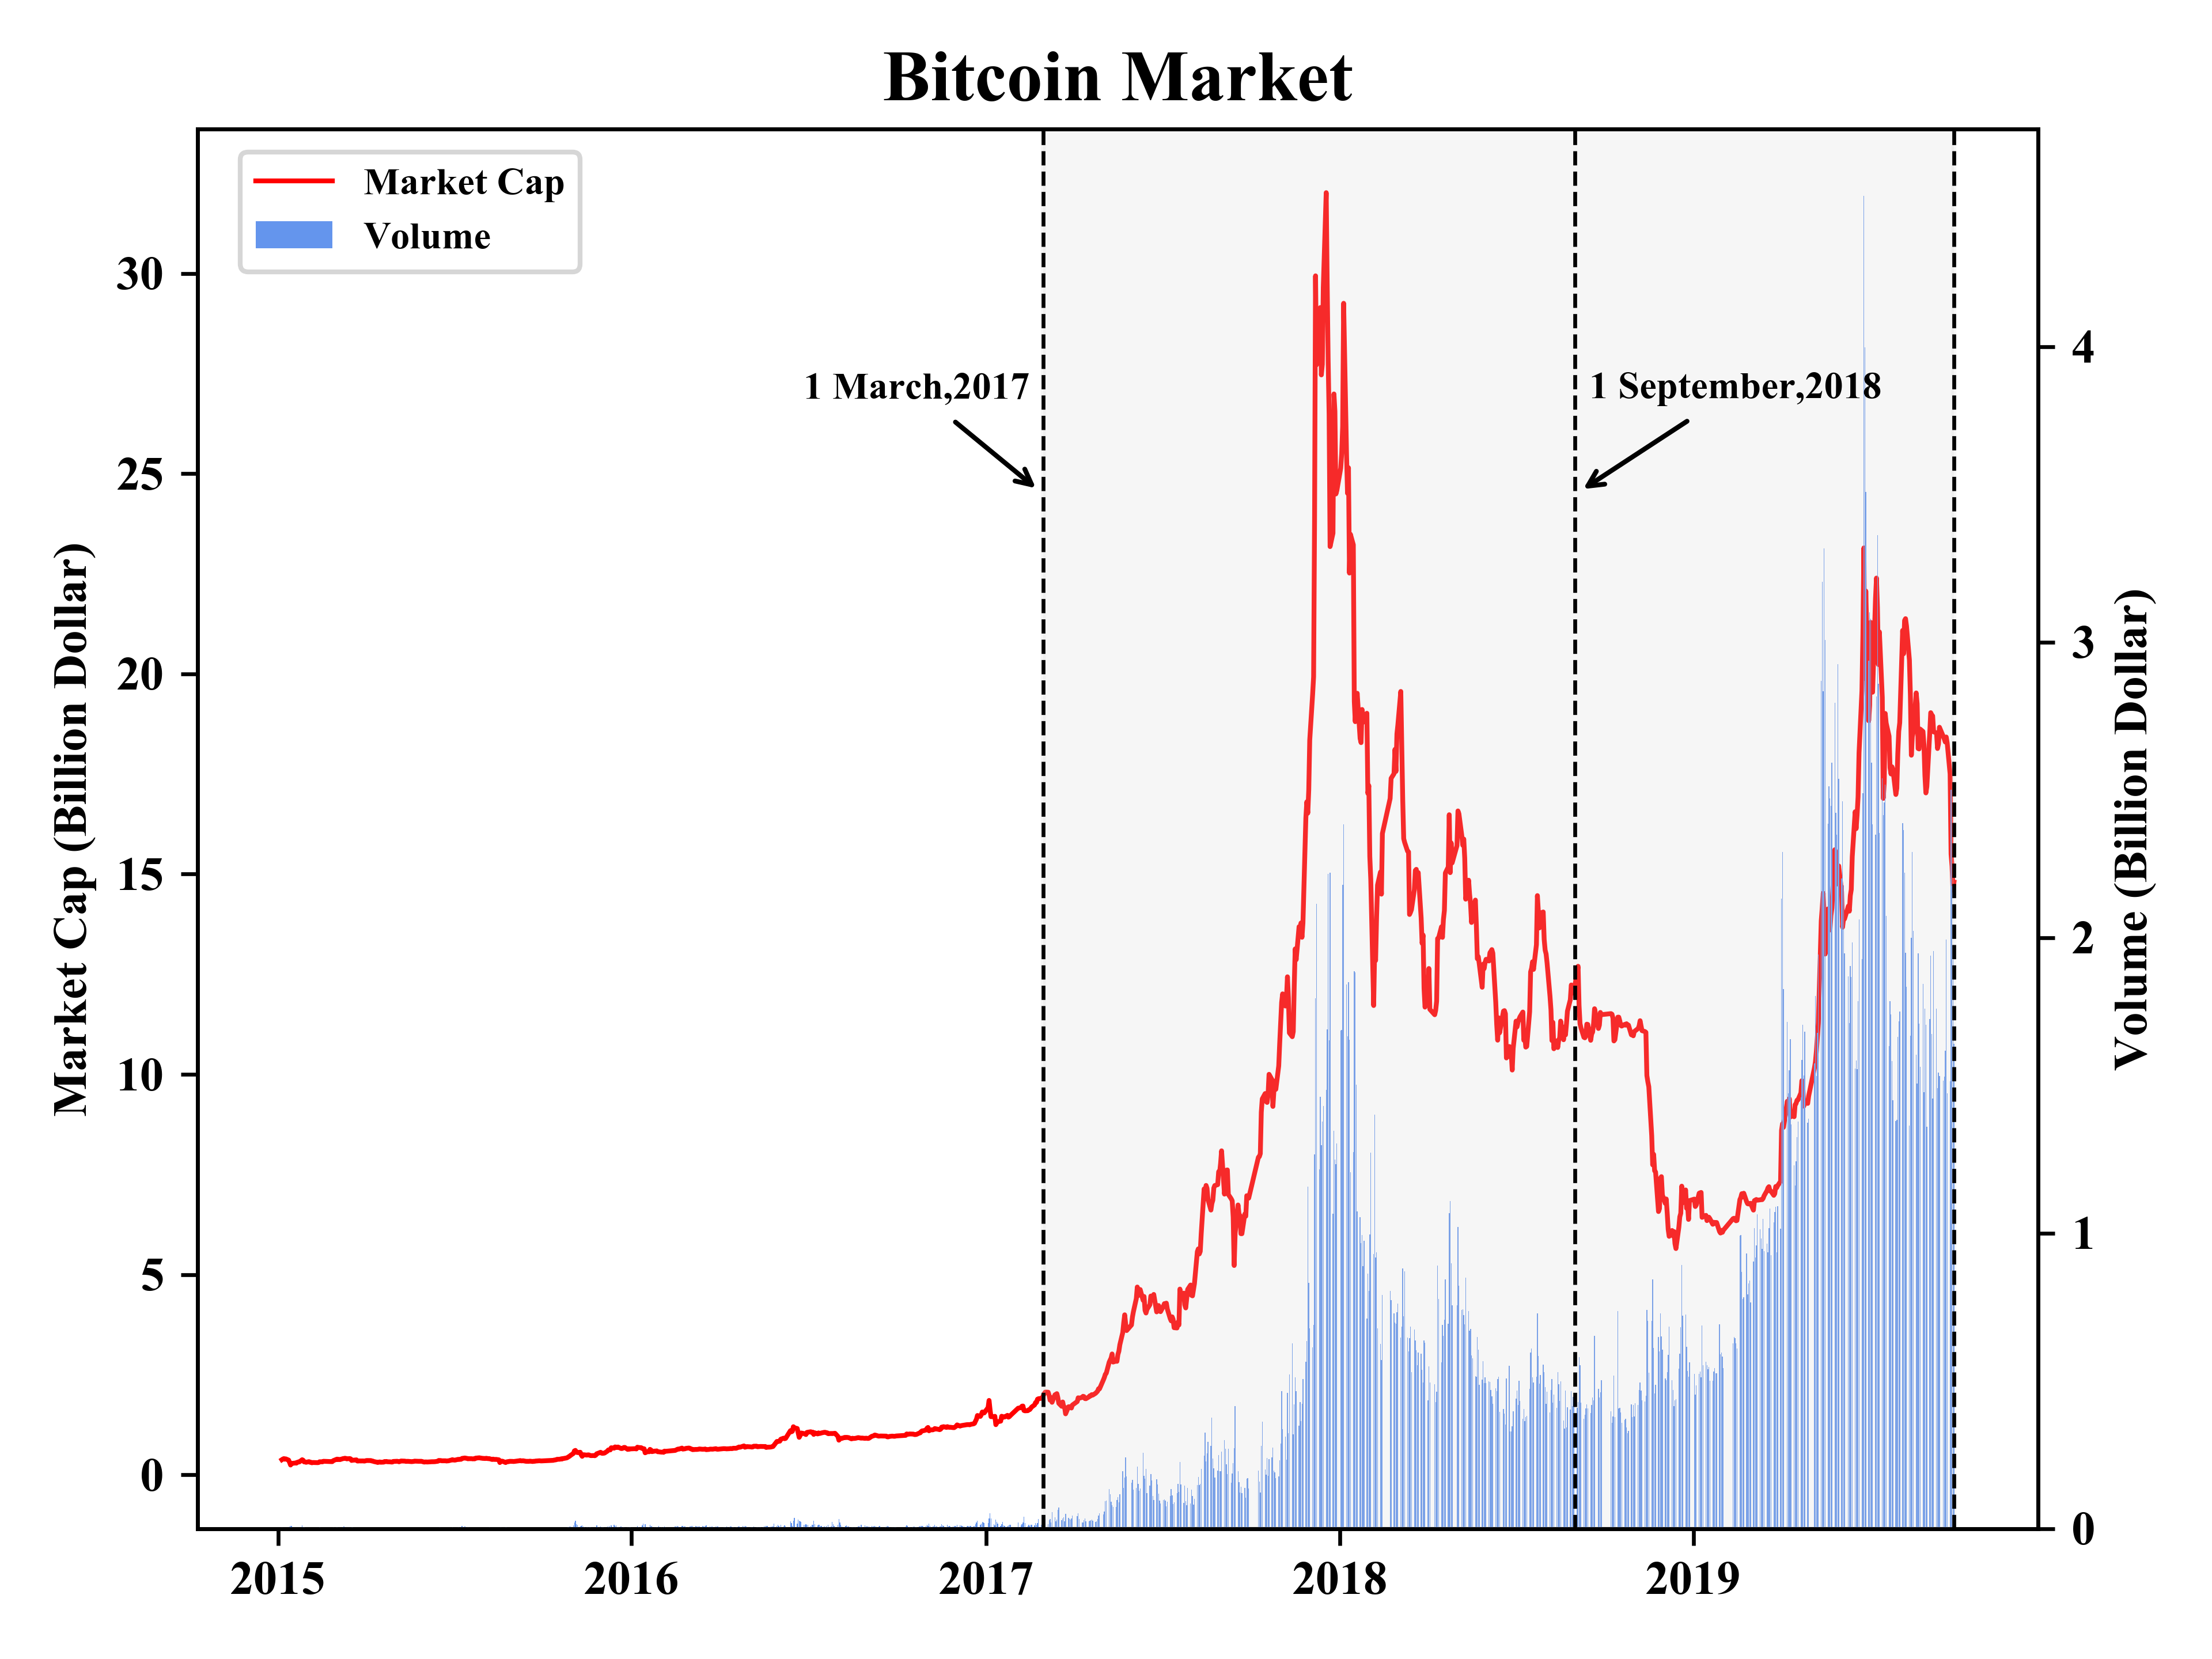
\includegraphics[scale=0.7]{BitcoinMarket.png}
	\caption{The daily market cap and volume of Bitcoin Market from 1 January,2014 to 27 September,2019}
	\label{img1}
\end{figure}

As Figure \ref{img1} shows, Bitcoin Market do not become buoyant until 2017. Therefore,the data spans the period 1 March, 2017 to 27 September, 2019, with a total of 633 daily observations. Moreover, two peaks appeared, which inspires us to analyze in stages. Considering China and the United States are the two largest economies in the world, we divide the entire sample into two periods in conjunction with the Sino-US trade dispute process. Since the 301 investigation on 18 August, 2017, Sino-US trade friction has been continuously upgraded.Noticing that the United States imposed 10\% tariff on 200 billion US dollars of products, accounting for 39.56\% of the total US imports from China on 24 September, 2018.\footnote{In 2017, the United States imported 505.60 billion US dollars from China. See \url{https://www.commerce.gov/}}Therefore, the whole period is bounded by September 2018. As demonstrated in Figure \ref{img1},the first period is from 1 March, 2017 to 31 August, 2018, and the second period is from 1 September, 2018 to 27 September, 2019 respectively.

\paragraph{Financial Market}For traditional financial market, we concentrate on stock, Forex and gold market. Moreover, our data covers the same period as Bitcoin(Figure \ref{img1}) in the WIND database.\footnote{In fact, although these markets have different opening time, we use the time series of HuShen 300 index in the WIND database.} More precisely, for gold market, four successful varieties are focused on, namely: International Spot Gold(ISG), International Futures Gold (IFG), Domestic Spot Gold (DSG) and Domestic Futures Gold (DFG).\footnote{London Metal Exchange:Loco London, COMEX:GC, ShangHai Futures Exchange:AU and ShangHai Futures Exchange:AU9999, respectively} For stock market, we interest in seven main stock markets in the world,namely: Standard \& Poor's 500-stock index(SP500) for the United States, the HuShen 300 index (SH300) and  the Hang Seng Index (HSI) for China, the FTSE 100 index (FTSE) for the United Kingdom, the Nikkei 225 index(N225) for Japan, the Germany’s DAX 30 (GDAXI) and CAC40 index (FCHI) for French. For currency market ,we use data of the global seven popular Forex currencies, namely:US Dollar Index (USDX), USD/CNY (UYE), USD/CNH (CNH), USD/HPY (UJE), EUR/USE (EUE), GBP/USD (GUE) and USD/CAD (UDE). In addition, francs, internationally recognized safe haven assets, are also taken into account. Actually, we use data of USD/CHF (UFE).

\subsubsection{Volatility Computation}
In the tradition of a large body of literature dating back at least to \cite{parkinson1980extreme}, we calculate the daily variance with daily high and low prices.For market $i$ on day $t$, we have the estimated daily variance

\begin{equation}
	\widetilde{\sigma}_{it}^2 = 0.361[ln(P_{it}^{max})-ln(P_{it}^{min})]^2
\end{equation}

Where $P_{it}^{max}$ is the daily maximum (high) price in market $i$ on day $t$, and $P_{it}^{min}$ is the daily minimum (low) price,respectively. Therefore, the corresponding estimate of the annualized daily percent standard deviation 

\begin{equation}
	\hat{\sigma}_{it}^2 = 100 \sqrt{365 \cdot \widetilde{\sigma}_{it}^2}
\end{equation}

In order to eliminate heteroscedasticity, we use the log volatility data in our study. For a more intuitive impression, we draw Bitcoin's Volatility and Volume in Figure \ref{img2}. Several interesting facts emerge, including: first of all, the volatility dynamics appear to be highly choppy; Secondly, the volume increases since the United States puts ``301 Investigation'' into practice. It is obvious that Bitcoin market is effected by Sino-US trade dispute. Finally,the volatility decreases when G20 summits held. As Figure \ref{img1} shows, market value, in particular, displays huge jumps in these days. Therefore, Bitcoin seems to be a safe haven asset, which will be carefully studied. 
 
\subsubsection{Descriptive Statistics and Test of Stationary}The summary statistics of all markets' volatilities is separately provided for stock,currency and gold markets in the sequential tables.Moreover, we also present the results of several tests, including:three methods for testing stationary\footnote{Namely, the Augmented Dickey-Fuller (ADF), Phillips-Perron (PP) and Kwiatkowski–Phillips–Schmidt–Shin (KPSS) test}, an algorithm for testing the normal distribution\footnote{Namely, the Jarque–Bera (J–B) test}, serial autocorrelation test \footnote{Namely, the Breusch-Godfrey (B-G) test} and ARCH effect test. 

\begin{figure}[htbp]		
	\centering
	\includegraphics[scale=0.7]{BitcoinVolatility.png}
	\caption{Daily Bitcoin market volatility and volume (annualized standard deviations,percentages)}
	\label{img2}
\end{figure}

\paragraph{Stock Markets}
Following Table \ref{tab1}, the daily mean volatility is 2.64 for SH300 and thus it is the largest volatility. However, the stock markets' daily mean volatilities have little difference, which may mean that information spreads quickly to smooth fluctuations in various markets.On the one hand, all values of skewness are positive. This positive sign is perceived to have a long tail to the right of distribution. Noting that the larger positive values of skewness are associated with the United States and Japan' stock indexes. Therefore, this prevent that there is a great chance that these stock markets little fluctuant, thus more efficient, during our sample period. On the other hand, combining skewness and kurtosis values, the volatility series showed a heavy tail for SH300, FTSE and GDAXI. This departure from normality is confirmed by the J-B test.


At the same time, the time series are proved to be stationary at 1\% level of significance for all samples. In addition, the results of B-G test reveals that all sequences are autocorrelation in the residuals from an $AR(1)$ regression model. Finally, ARCH effect does not exist.


\begin{table}[]
	\centering
	\setlength{\abovecaptionskip}{0pt}%    
	\setlength{\belowcaptionskip}{10pt}%
	\caption{Summary statistics of daily volatility related to stock markets \footnotemark}
	\label{tab1}
	\scalebox{0.65}{
	\begin{tabular}{ccccccccc}
		\hline
		& SP500 & NASDAQ & SH300 & N225 & FTSE & GDAXI & FCHI & HSI \\
		\hline
		Mean & 2.11 & 2.36 & 2.64 & 2.22 & 2.29 & 2.38 & 2.29 & 2.45 \\
		Median & 2.04 & 2.28 & 2.62 & 2.17 & 2.3 & 2.38 & 2.27 & 2.43 \\
		Maximum & 4.06 & 4.12 & 3.89 & 4.15 & 3.74 & 3.67 & 3.52 & 3.78 \\
		Minimum & 0.51 & 0.92 & 1.39 & 0.8 & 1.02 & 0.83 & 1.11 & 1.35 \\
		Std.Deviation & 0.65 & 0.61 & 0.49 & 0.49 & 0.45 & 0.48 & 0.46 & 0.43 \\
		Skewness & 0.45 & 0.36 & 0.12 & 0.36 & 0.06 & 0.04 & 0.17 & 0.13 \\
		Kurtosis & 2.95 & 2.87 & 2.67 & 3.29 & 2.97 & 2.79 & 2.64 & 2.63 \\
		ADF & -11.125*** & -12.317*** & -15.484*** & -14.953*** & -16.764*** & -17.899*** & -16.734*** & -17.309*** \\
		PP & -11.492*** & -13.025*** & -17.104*** & -16.028*** & -18.256*** & -19.711*** & -18.073*** & -19.003*** \\
		KPSS & 1.39*** & 1.37*** & 2.38*** & -2.01*** & 0.672*** & 1.04*** & 0.305*** & 2.42*** \\
		J-B & 21.15*** & 14.26*** & 4.36 & 15.74*** & 0.34 & 1.31 & 6.358** & 5.295* \\
		B-G & 64.793*** & 55.655*** & 64.096*** & 30.054*** & 28.700*** & 42.366*** & 24.758*** & 35.455*** \\
		ARCH-LM & 0.35 & 0.16 & 0.54 & 0.11 & 1.32 & 0.05 & 0.06 & 0.6\\
		\hline
	\end{tabular}
}
\end{table}
\footnotetext{$*$, $**$ and $***$ denote significance at 10\%, 5\% and 1\%, respectively, which will not be repeated in the rest of the article}

\paragraph{Currency Markets}
As Table \ref{tab2} shows, China's currency exchanges, including UYE and CNH, have smaller mean volatility while the GBP has a top volatility in the average sense. Unlike stock indices, the volatilities of currency exchanges are perceived to have a long tail to the left from sign of skewness. Furthermore, it is confirmed that UYE and CNH deviate from normality, which means that the data has a heavy tail.


The time series are also significantly stationary for all test methods. In another term, the result of B-G test indicates that the absence of autocorrelation in the residuals from an $AR(1)$ model for USDX. More interestingly, we can observe that five sequences have ARCH effect at 1\% level of confidence, which provides a robustness test for our study. 


\begin{table}[]
	\centering
	\setlength{\abovecaptionskip}{0pt}%    
	\setlength{\belowcaptionskip}{10pt}%
	\caption{Summary statistics of daily volatility related to currency markets}
	\label{tab2}
	\scalebox{0.65}{
	\begin{tabular}{ccccccccc}
		\hline
		& USDX & UYE & EUE & UJE & GUE & UDE & UFE & CNH \\
		\hline
		Mean & 1.73 & 1.12 & 1.88 & 1.89 & 2.07 & 1.87 & 1.87 & 1.41 \\
		Median & 1.76 & 1.11 & 1.95 & 1.95 & 2.08 & 1.89 & 1.9 & 1.4 \\
		Maximum & 3.07 & 2.68 & 3.34 & 3.77 & 3.57 & 3.15 & 3.08 & 3.06 \\
		Minimum & -1.49 & -0.44 & -2.31 & -2.94 & -1.75 & -1.75 & -2.16 & -0.92 \\
		Std.Deviation & 0.46 & 0.58 & 0.56 & 0.57 & 0.52 & 0.53 & 0.53 & 0.55 \\
		Skewness & -1.86 & -0.06 & -3.03 & -2.75 & -2.42 & -2.28 & -2.53 & 0.01 \\
		Kurtosis & 13.92 & 2.73 & 21.25 & 21 & 18.03 & 15.29 & 18.03 & 3.17 \\
		ADF & -22.709*** & -12.578*** & -20.718*** & -19.426*** & -20.764*** & -22.115*** & -18.606*** & -14.484*** \\
		PP & -23.286*** & -13.055*** & -21.761*** & 20.477*** & -21.600*** & -22.820*** & -19.341*** & -15.321*** \\
		KPSS & 0.602*** & 3.22*** & 0.617*** & 0.141* & 0.224*** & 0.564*** & 0.308*** & 1.98*** \\
		J-B & 3509*** & 2.29 & 9750*** & 9345*** & 6581*** & 4529*** & 6635*** & 0.79 \\
		B-G & 1.88 & 11.930*** & 23.151*** & 22.526*** & 23.375*** & 16.047*** & 5.690** & 8.310*** \\
		ARCH-LM & 0.02 & 0.51 & 10.110*** & 69.678*** & 22.904*** & 11.429*** & 42.438*** & 0.25\\
		\hline
	\end{tabular}
}
\end{table}

\paragraph{Gold Markets}
Regardless of the future or spot market, the Table \ref{tab3} demonstrates that international gold markets have a higher average of daily volatility during our sample period. Additionally, noting that Bitcoin has a top daily mean volatility covering all the data,including stock markets and currency markets.The different sign of skewness show that Bitcoin and SIG have a left tail.However, J-B test reveals that all data are normally distributed. 


The stationarity is also confirmed. In addition, all data is autocorrelation under the sense of residuals from an $AR(1)$ model except for FIG series.Furthermore, the ARCH effect is absence in the gold market. In conclusion, Bitcoin almost passes all the test in this paper, including ARCH-LM test.


\begin{table}[]
	\centering
	\setlength{\abovecaptionskip}{0pt}%    
	\setlength{\belowcaptionskip}{10pt}%
	\caption{Summary statistics of daily volatility related to gold markets}
	\label{tab3}
	\scalebox{0.65}{
	\begin{tabular}{cccccc}
		\hline
		& Bitcoin & ISG & IFG & DFG & DSG \\
		\hline
		Mean & 3.94 & 2.39 & 2.41 & 1.96 & 2.13 \\
		Median & 3.99 & 2.38 & 2.39 & 1.9 & 2.07 \\
		Maximum & 5.86 & 3.74 & 3.77 & 3.75 & 4.37 \\
		Minimum & 1.77 & -2 & 1.36 & 0.85 & 0.8 \\
		Std.Deviation & 0.75 & 0.47 & 0.4 & 0.52 & 0.56 \\
		Skewness & -0.17 & -1.67 & 0.3 & 0.74 & 0.82 \\
		Kurtosis & 2.72 & 17.08 & 2.96 & 3.73 & 4.37 \\
		ADF & -13.174*** & -21.992*** & -21.977*** & -15.461*** & -17.098*** \\
		PP & -14.072*** & -22.835*** & -22.884*** & -16.744*** & -18.401*** \\
		KPSS & 1.62*** & 0.79*** & 0.817*** & 3.64*** & 3.06*** \\
		J-B & 5.084* & 5524*** & 9.849*** & 71.91*** & 120.1*** \\
		B-G & 52.318*** & 9.152*** & 0.99 & 14.999*** & 23.611*** \\
		ARCH-LM & 8.473*** & 0 & 0.28 & 0.17 & 0.92\\
		\hline
	\end{tabular}
}
\end{table}


\subsection{Methodology}
Two quite different methods were used to measure the connectedness between two markets, including the GARCH family model, such as \cite{Baur2018,Vidal-Tomas2018,symitsi2018return}, and the framework based on variance decomposition, such as \cite{trabelsi2018there,awartani2013dynamic}.


\subsubsection{Generalized Variance Decomposition}
We begin with a covariance stationary \emph{N}-variable \emph{VAR(p)}

\begin{equation}
	\chi_t = \sum\limits_{i=1}^n \Phi_i \chi_i + \varepsilon_i 
\end{equation}

Where $\varepsilon_i \sim (0, \sum)$ is a vector of independently and identically distributed disturbances. Then the moving average representation is defined as

\begin{equation}
	\chi_t = \sum \limits_{k=1}^\infty A_i \varepsilon_i 
\end{equation}

Where the $N \times N$ coefficient matrices $A_i$ obey the recursion $A_i = \Phi_1 A_{i-1} +\Phi_2 A_{i-2} + \cdots + \Phi_p A_{p-1}$, with $A_0$ being an $N \times N$ identity matrix and with $A_i=0$ for $i < 0$. This moving average coefficient, (called also variance decomposition or impulse response function) are essential to grasp the dynamic system. With exploiting the generalized \emph{VAR} framework to calculate the variance decomposition proposed by \cite{Koop1996, pesaran1998generalized} hereafter \emph{KPPS}, the problem that depends on the order of the variables is perfectly circumvented. Hence, we will parse the spillover from the perspective of variance decomposition.

\paragraph{Variance Shares} Starting at proposing two essential definition. With the $H$-step-ahead error variance in forecasting $\Phi_i$, we define \emph{own variance shares} as the fractions that due to shocks to $\Phi_i$, for $i=1,2.\cdots,N$, and \emph{cross variance shares, or spillover}, as the fractions that due shocks to $\Phi_j$ for $i,j=1,2,\cdots,N$, such that $i \neq j$.

Therefore, noticing the \emph{KPPS} $H$-step ahead forecast error variance decomposition $\theta_{ij}^g (H)$, for $H=1,2,\cdots,N$ defined as

\begin{equation}
\[
 	\theta_{ij}^g (H) = \frac{\sigma_{jj}^{-1} \sum\limits_{h=0}^{H-1} ({e_i^'} A_h \Sigma e_j)^2}{\sum\limits_{h=0}^{H-1} ({e_i^'} A_h \Sigma {A_h^'} e_i)}
\]
\end{equation}

Where $\sum$ is the variance matrix for the error vector $\varepsilon$, $\sigma_{jj}$ is the standard deviation of the error term for the \emph{j} th equation, and $e_i$ is the selection vector. \footnote{Namely, one as the \emph{i}th and zero otherwise.} In addition, since the shock to each variable are not orthogonalized, the sum of this contributions is not necessarily equal to one, or rather: $\sum\limits_{j=1}^N \theta_{ij}^g (H) \ne 1$. Furthermore, in order to make full use of information available in the variable decomposition matrix in calculating spillover index, we normalize each entry of the variance decomposition matrix by the row sum. 

\begin{equation}
	\widetilde{\theta}_{ij}^g (H) = \frac{\theta_{ij}^g (H)}{\sum\limits_{j=1}^H \theta_{ij}^g (H)}
\end{equation}

As construction indicates, $\sum_{j=1}^{N} \widetilde{\theta}_{ij}^g (H) = 1$ and $\sum_{i,j=1}^{N} \widetilde{\theta}_{ij}^g (H) = N$.

\paragraph{Directional Spillover}
The purpose of this paper is to measure the directional shocks and connectedness. Therefore, based on the invariance of the ordering of variables for the generalized impulse responses and variance decomposition, we calculate the directional spillovers using the normalized elements of the generalized variance decomposition matrix. And we measure the directional volatility spillover received by market \emph{i} form all other markets \emph{j} as below
\begin{equation}
	\label{FROM}
	S_{i \rightarrow}^g (H) = \frac{\sum\limits_{j=1,j \ne i}^N \widetilde{\theta}_{ij}^g (H)}{\sum\limits_{i,j=1}^N \widetilde{\theta}_{ij}^g (H)} \cdot 100 
\end{equation}

On the contrary, we measure the directional volatility spillover transmitted by market \emph{i} to all other markets \emph{j} as below
\begin{equation}
	\label{TO}
	S_{\rightarrow i}^g (H) = \frac{\sum\limits_{j=1,j \ne i}^N \widetilde{\theta}_{ji}^g (H)}{\sum\limits_{i,j=1}^N \widetilde{\theta}_{ji}^g (H)} \cdot 100 
\end{equation}

\paragraph{Net Volatility  Spillover and Connetedness}
We have obtained the bidirectional spillover of market \emph{i} ``TO'' and ``FROM'' the other markets \emph{j}, and the net volatility spillover is naturally defined as
\begin{equation}
	\label{NetSpillover}
	S_i^g (H) = S_{\rightarrow i}^g (H) - S_{i \rightarrow}^g (H)
\end{equation}

The connectedness reveals that two markets are mutually affected, which combines the bidirectional influence. Therefore, we define the geometric mean of bidirectional disturbance as the connection intensity, namely
\begin{equation}
	\label{Conetedness}
	C_{i}^g = \sqrt{ S_{\rightarrow i}^g (H) \cdot S_{i \rightarrow}^g (H)}\
\end{equation}

It is worth noting that while the studied objects concentrate on individual two markets, Equation \ref{NetSpillover} and Equation \ref{Conetedness} actually describe the mutual connectedness among the two interested markets.


\subsubsection{The DCC-GARCH Model}
Then, we turn to describe the DCC-GARCH model \cite{Engle2002}. Assuming that $\varepsilon_t (N \time 1)$ is the innovation process for the conditional mean and can be written as

\begin{equation}
	\varepsilon_t | \Psi_{t-1} \sim LG(0,\Sigma_t)
\end{equation}

Where $\Phi_{t-1}$ is the set of all information available at time \emph{t-1}, LG is the multivariate Laplace-Gaussian distribution (called also multivariate normal distribution) and $\Sigma_t$ is the $N \times N$ symmetric conditional covariance matrix. Hence, the $\emph{DCC(P,Q)-GARCH(p,q)}$ by \cite{Engle2002} can be presented as below
\begin{equation}
	\Sigma_t = \Lambda_t \Omega_t \Lambda_t 
\end{equation}
\begin{equation}
	\Omega_t = \widetilde{\Phi}_t^{-1} \Phi_t \widetilde{\Phi}_t^{-1}
\end{equation}
\begin{equation}
\[
	\Phi_t = (1-\sum\limits_{i=1}^Q \xi_i - \sum\limits_{j=1}^P \theta_j ) \Psi + \sum\limits_{i=1}^Q \xi_i (z_{t-i}{z_{t-i}^'}) + \sum\limits_{i=1}^P \theta_j \Phi_{t-j}
\]
\end{equation}

Where $\Lambda_t = diag(h_{1t}^{1/2}, h_{2t}^{1/2}, \cdots, h_{Nt}^{1/2})$, and the conditional variances $h_{kt} = \alpha_{k0} + \sum_{i=1}^q \aleph_{k,i} \varepsilon_{k,t-i}^2 + \sum_{j=1}^p \beta_{k,j} h_{k,t-j}^2$ (for $k = 1,2, \dots, N$) is an univariate GARCH model. Subsequently, $z_t$ is the standardized $N \times 1$ residual vector assumed to be serially in dependently distributed given as $z_t = \Lambda_t^{-1} \varepsilon_t$, and $\Omega_t$ is the time varying $N \times N$ conditional matrix of $z_t$. In addition, $\Psi$ is the unconditional $N \times N$ covariance matrix of $z_t$. Finally, $ \widetilde{\Phi}_t$ is the diagonal $N \times N$ matrix composed of the square root of the diagonal elements of $\Phi_t$ and the parameters, such as $\x_i$ and $\theta_j$ (for $i=1,2,\cdots,Q$ and $j=1,2,\cdots,P$) are nonnegative and satisfy a constraint condition $\sum_{i=1}^Q \xi_i + \sum_{j=1}^P \theta_j < 1$.

Noticing that DCC-GARCH model is only appropriate to the case that the data passed the ARCH effect test. Therefore, we use DCC-GARCH model for testing the robustness due to the absence of ARCH effect in some data.


\subsubsection{Summary of Methodology}
In this paper, we mainly make use of the generalized variance decomposition model to study the relationship between cruptocurrency markets and other traditional financial markets. In addition, DCC-GARCH model and Pearson Correlation is adopted to check the robustness. Finally, we also apply Granger-Cause method to clarify the direction of disturbance, which should be corresponding with Equation \ref{TO} and Equation \ref{FROM}. Based on these potent techniques, some insightful conclusion will be naturally emerged. 


\section{Empirical Findings and Discussion}
With measuring the volatility spillovers of Bitcoin on other asset classes in detail, we elaborate the connectedness, dependence and mutual effect. More interestingly, comparing these conclusions, the significant driving force of Bitcoin will be revealed.


The remainder of this section as follows.We begin by comparing the volatilities over all sample in stages, which shows the concerned targets.Subsequently, we will concentrate on the worthy objects, which brings the main conclusions.Lastly, robustness analysis will be reported. \footnote{Since all tests are significant under 1th lag intervals for endogenous, our studies are also based on order 1, including generalized variance decomposition, DCC-GARACH and Granger-Cause test. In addition, we calculate 5-day-ahead volatility forecast errors. The other orders are also calculated, we do not report due to space limitation.}

\subsection{Full Sample Performances}
The volatility spillover of Bitcoin TO/FROM other asset classes is displayed on Table \ref{tab4}. ``All Sampl'' represents the full-sample period. ``First Stage'' and ``Second Stage'' denotes the epoch from 1 March, 2017 to 31 August, 2018, and from 1 September, 2018 to 27 September, 2019, respectively. As a matter of fact, the approximate ``input-output'' decomposition of the total volatility spillover is reported in this table. 

\begin{table}[]
	\centering
	\setlength{\abovecaptionskip}{0pt}
	\setlength{\belowcaptionskip}{10pt}
	\caption{Volatility spillover of Bitcoin TO/FROM asset classes}
	\label{tab4}
	\renewcommand\tabcolsep{10 pt}
	\scalebox{0.65}{
		\begin{tabular}{cccccccccccc}
			\hline
			& \multicolumn{11}{c}{Bitcoin} \\
			\cline{2-12}
			& \multicolumn{3}{c}{Full Sample} &  & \multicolumn{3}{c}{First Stage} &  & \multicolumn{3}{c}{Second Stage} \\
			\cline{2-4}
			\cline{6-8}
			\cline{10-12}
			& To & From & Total &  & To & From & Total &  & To & From & Total \\
			\hline
			IFG & 0.36 & 0.83 & 0.55 &  & 0.08 & 0.07 & 0.07 &  & 1.46 & 3.64 & 2.31 \\
			ISG & 0.26 & 0.78 & 0.45 &  & 0.08 & 0.07 & 0.07 &  & 0.76 & 2.41 & 1.35 \\
			DSG & 0.05 & 0.47 & 0.15 &  & 0.19 & 0.27 & 0.23 &  & 0.68 & 0.33 & 0.47 \\
			DFG & 0.11 & 0.16 & 0.13 &  & 0.11 & 0.02 & 0.05 &  & 1.71 & 3.06 & 2.29 \\
			SH300 & 1.57 & 0.90 & 1.19 &  & 0.07 & 0.21 & 0.12 &  & 3.37 & 1.45 & 2.21 \\
			HSI & 0.4 & 1.28 & 0.72 &  & 0.31 & 1.08 & 0.58 &  & 0.61 & 1.34 & 0.9 \\
			FTSE & 0.22 & 0.71 & 0.40 &  & 0.09 & 0.66 & 0.24 &  & 0.15 & 0.34 & 0.23 \\
			N225 & 0.15 & 0.61 & 0.30 &  & 0.77 & 0.03 & 0.15 &  & 0.66 & 1.83 & 1.1 \\
			GDAXI & 0.15 & 0.34 & 0.23 &  & 0.47 & 0.83 & 0.62 &  & 0.02 & 0.16 & 0.06 \\
			NASDAQ & 0.08 & 0.26 & 0.14 &  & 0.1 & 0.12 & 0.11 &  & 0.25 & 0.69 & 0.42 \\
			SP500 & 0.07 & 0.12 & 0.09 &  & 0.18 & 0.29 & 0.23 &  & 0.3 & 1.41 & 0.65 \\
			FCHI & 0.04 & 0.05 & 0.04 &  & 0.44 & 0.53 & 0.48 &  & 0.15 & 0.41 & 0.25 \\
			UFE & 1.00 & 3.03 & 1.74 &  & 1.07 & 3.65 & 1.98 &  & 0.2 & 0.68 & 0.37 \\
			UJE & 0.93 & 0.73 & 0.82 &  & 0.26 & 0.37 & 0.31 &  & 0.87 & 0.9 & 0.88 \\
			EUE & 0.33 & 1.26 & 0.64 &  & 0.03 & 0.72 & 0.15 &  & 0.73 & 1.44 & 1.03 \\
			UDE & 0.33 & 0.91 & 0.55 &  & 0.19 & 0.48 & 0.3 &  & 0.34 & 0.59 & 0.45 \\
			USDX & 0.28 & 0.64 & 0.42 &  & 0.03 & 0.5 & 0.12 &  & 0.78 & 0.99 & 0.88 \\
			GUE & 0.10 & 0.17 & 0.13 &  & 0.55 & 2.74 & 1.23 &  & 1.39 & 3.14 & 2.09 \\
			CNH & 0.07 & 0.14 & 0.10 &  & 0.09 & 0.2 & 0.13 &  & 0.05 & 0.04 & 0.04 \\
			UYE & 0.13 & 0.08 & 0.10 &  & 0.21 & 0.12 & 0.16 &  & 0.08 & 0.11 & 0.09 \\
			SUM & 6.63 & 13.47 & 8.89 &  & 5.32 & 12.96 & 7.33 &  & 14.56 & 24.96 & 18.07 \\
			\hline
		\end{tabular}
	}
\end{table}

Considering first the performances during full-sample period, severe interesting conclusions are revealed.On the one hand, among all markets, SH300 receives the top impact $( 1.57 / 6.62 = 23.72\%)$ and UFE contributes the biggest influence $( 3.03 / 13.45 = 22.53\%)$, respectively. On the other hand, from the comprehensive perspective, international gold assets (ISG and IFG) are closely related with Bitcoin for gold markets.In addition, China's stock markets (SH300 and HSI) are highly correlated for stock markets, which may emerge that Chinese investors use Bitcoin for hedging in that China's investors prefer Bitcoin than the US dollars during Sino-US trade dispute. Furthermore, we argue that Bitcoin has not being dollarized from the volatility spillover values of USDX among Forex markets \cite{DongGuo2019Dollarization}. On the contrary, we observe that Bitcoin has no national monetization in the case of watching JPY and the Franc ( UFE and UJE ) as a safe haven currency. 


We also find that China's currencies, including offshore and onshore RMB, are little effected by Bitcoin. Several possible explanations are proposed.Firstly, Bitcoin is not a legal trading currency in China, and RMB cannot be used directly for trading.Subsequently, RMB is not freely convertible because China' financial market are not fully open.Last but not least, trade in goods accounts for most of China's foreign trade, so the capital movement is weakly related to Bictoin's trend.More interestingly, the United States' stock markets (SP500 and NASDAQ), the most developed capital market in the world, are astoundingly little correlated with Bitcoin.

\subsection{Staged Performances}
Referring to Table \ref{tab4}, we now turn to study the volatility spillover changes during two different stages.With comparing these varieties in detail, meaningful conclusions are demonstrated from three perspectives.On the whole, the connectedness between Bitcoin and the other assets Dramatically increases in the second stage.In effect, the entire volatility spillover increases from 5.31\% to 14.57\% for ``To'' direction and from 12.98\% to 24.96\% for the opposite direction.

\subsubsection{Hedge Driving}
For gold market, future assets (IFG and DFG) and international spot golds (ISG) shows a sharp rise in the second stage. In fact, the volatilities of three assets increase from 1.23\% to 36.50\% for ``From'' direction and from 5.08\% to 26.97\% for another direction, which means that the relatedness between Bitcoin and gold assets increase dramatically after 200 billion US dollars tariff. Additionally, with focusing on future assets, investors are mainly worried about the prospective uncertainties of Sino-US trade dispute. Therefore, the investors use futures for hedging the nondeterminacy in time. It is obvious that Bitcoin has becomes a safe haven asset because of the high connectedness.


\begin{figure}[H]
	\centering  %图片全局居中
	\subfigure[Correlation of IFG]{
		\label{Gold.sub.1}
		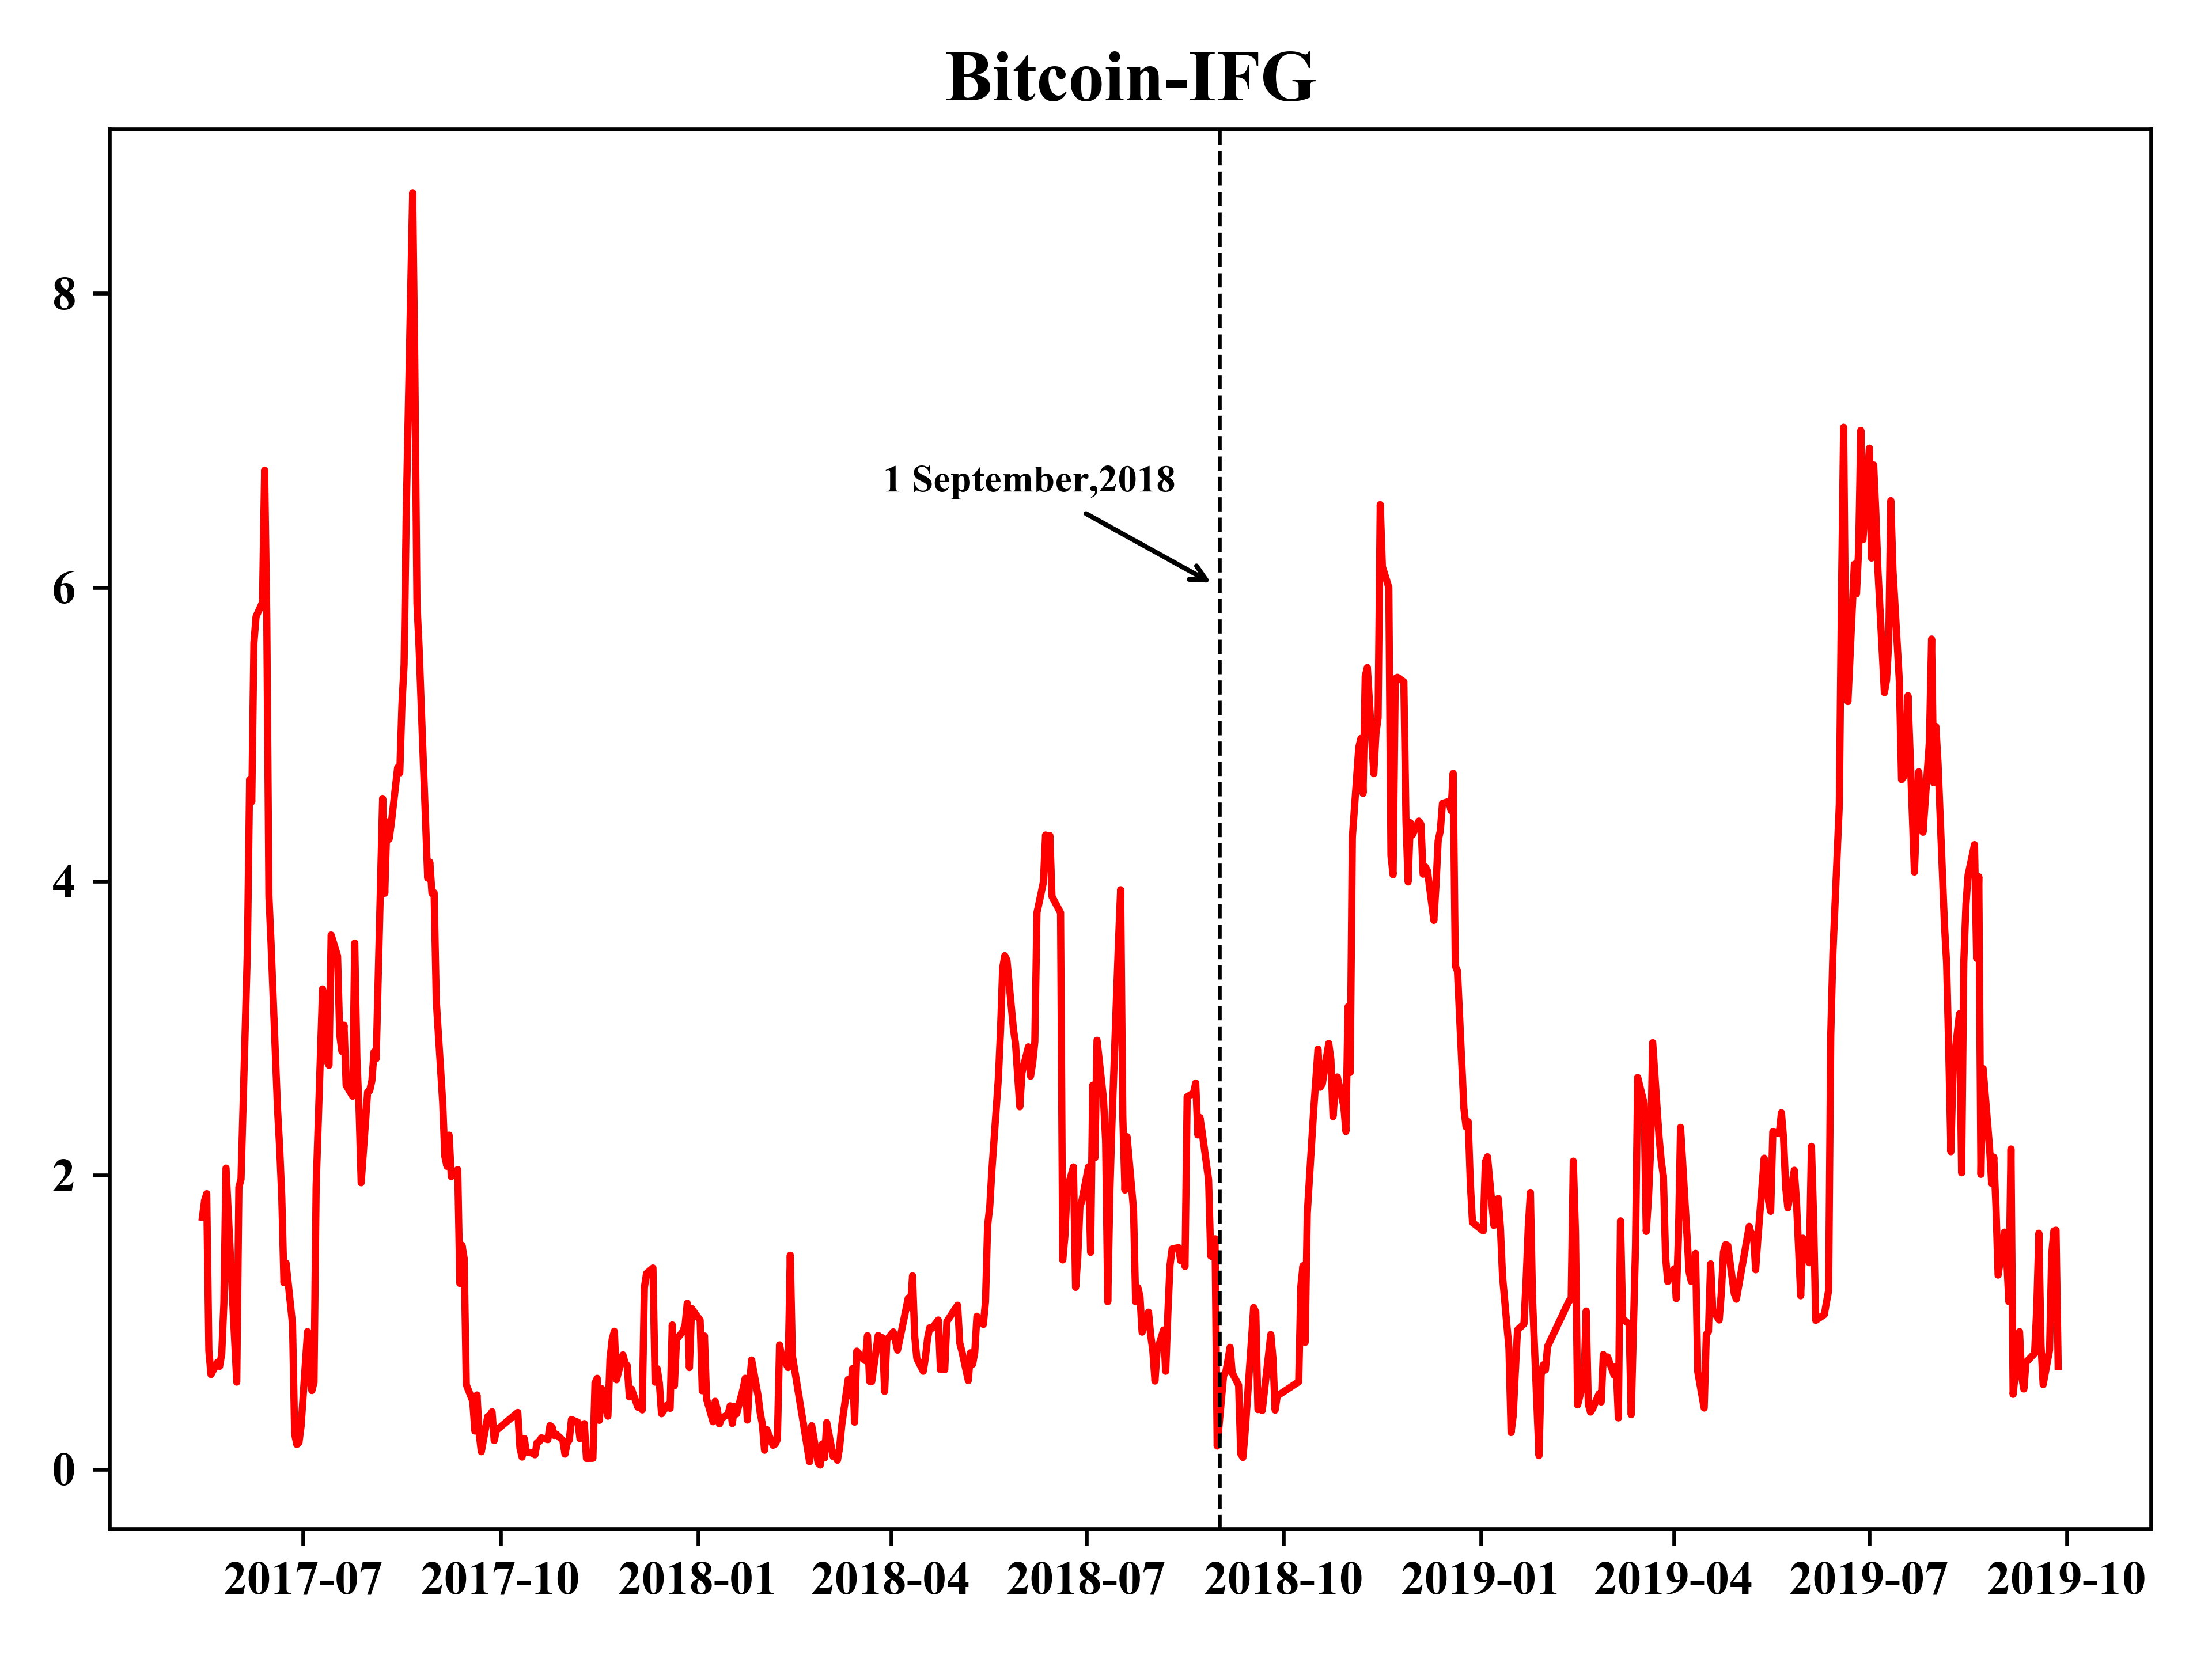
\includegraphics[width=0.45\textwidth]{IFG.png}}
	\subfigure[NPVS of IFG]{
		\label{Gold.sub.2}
		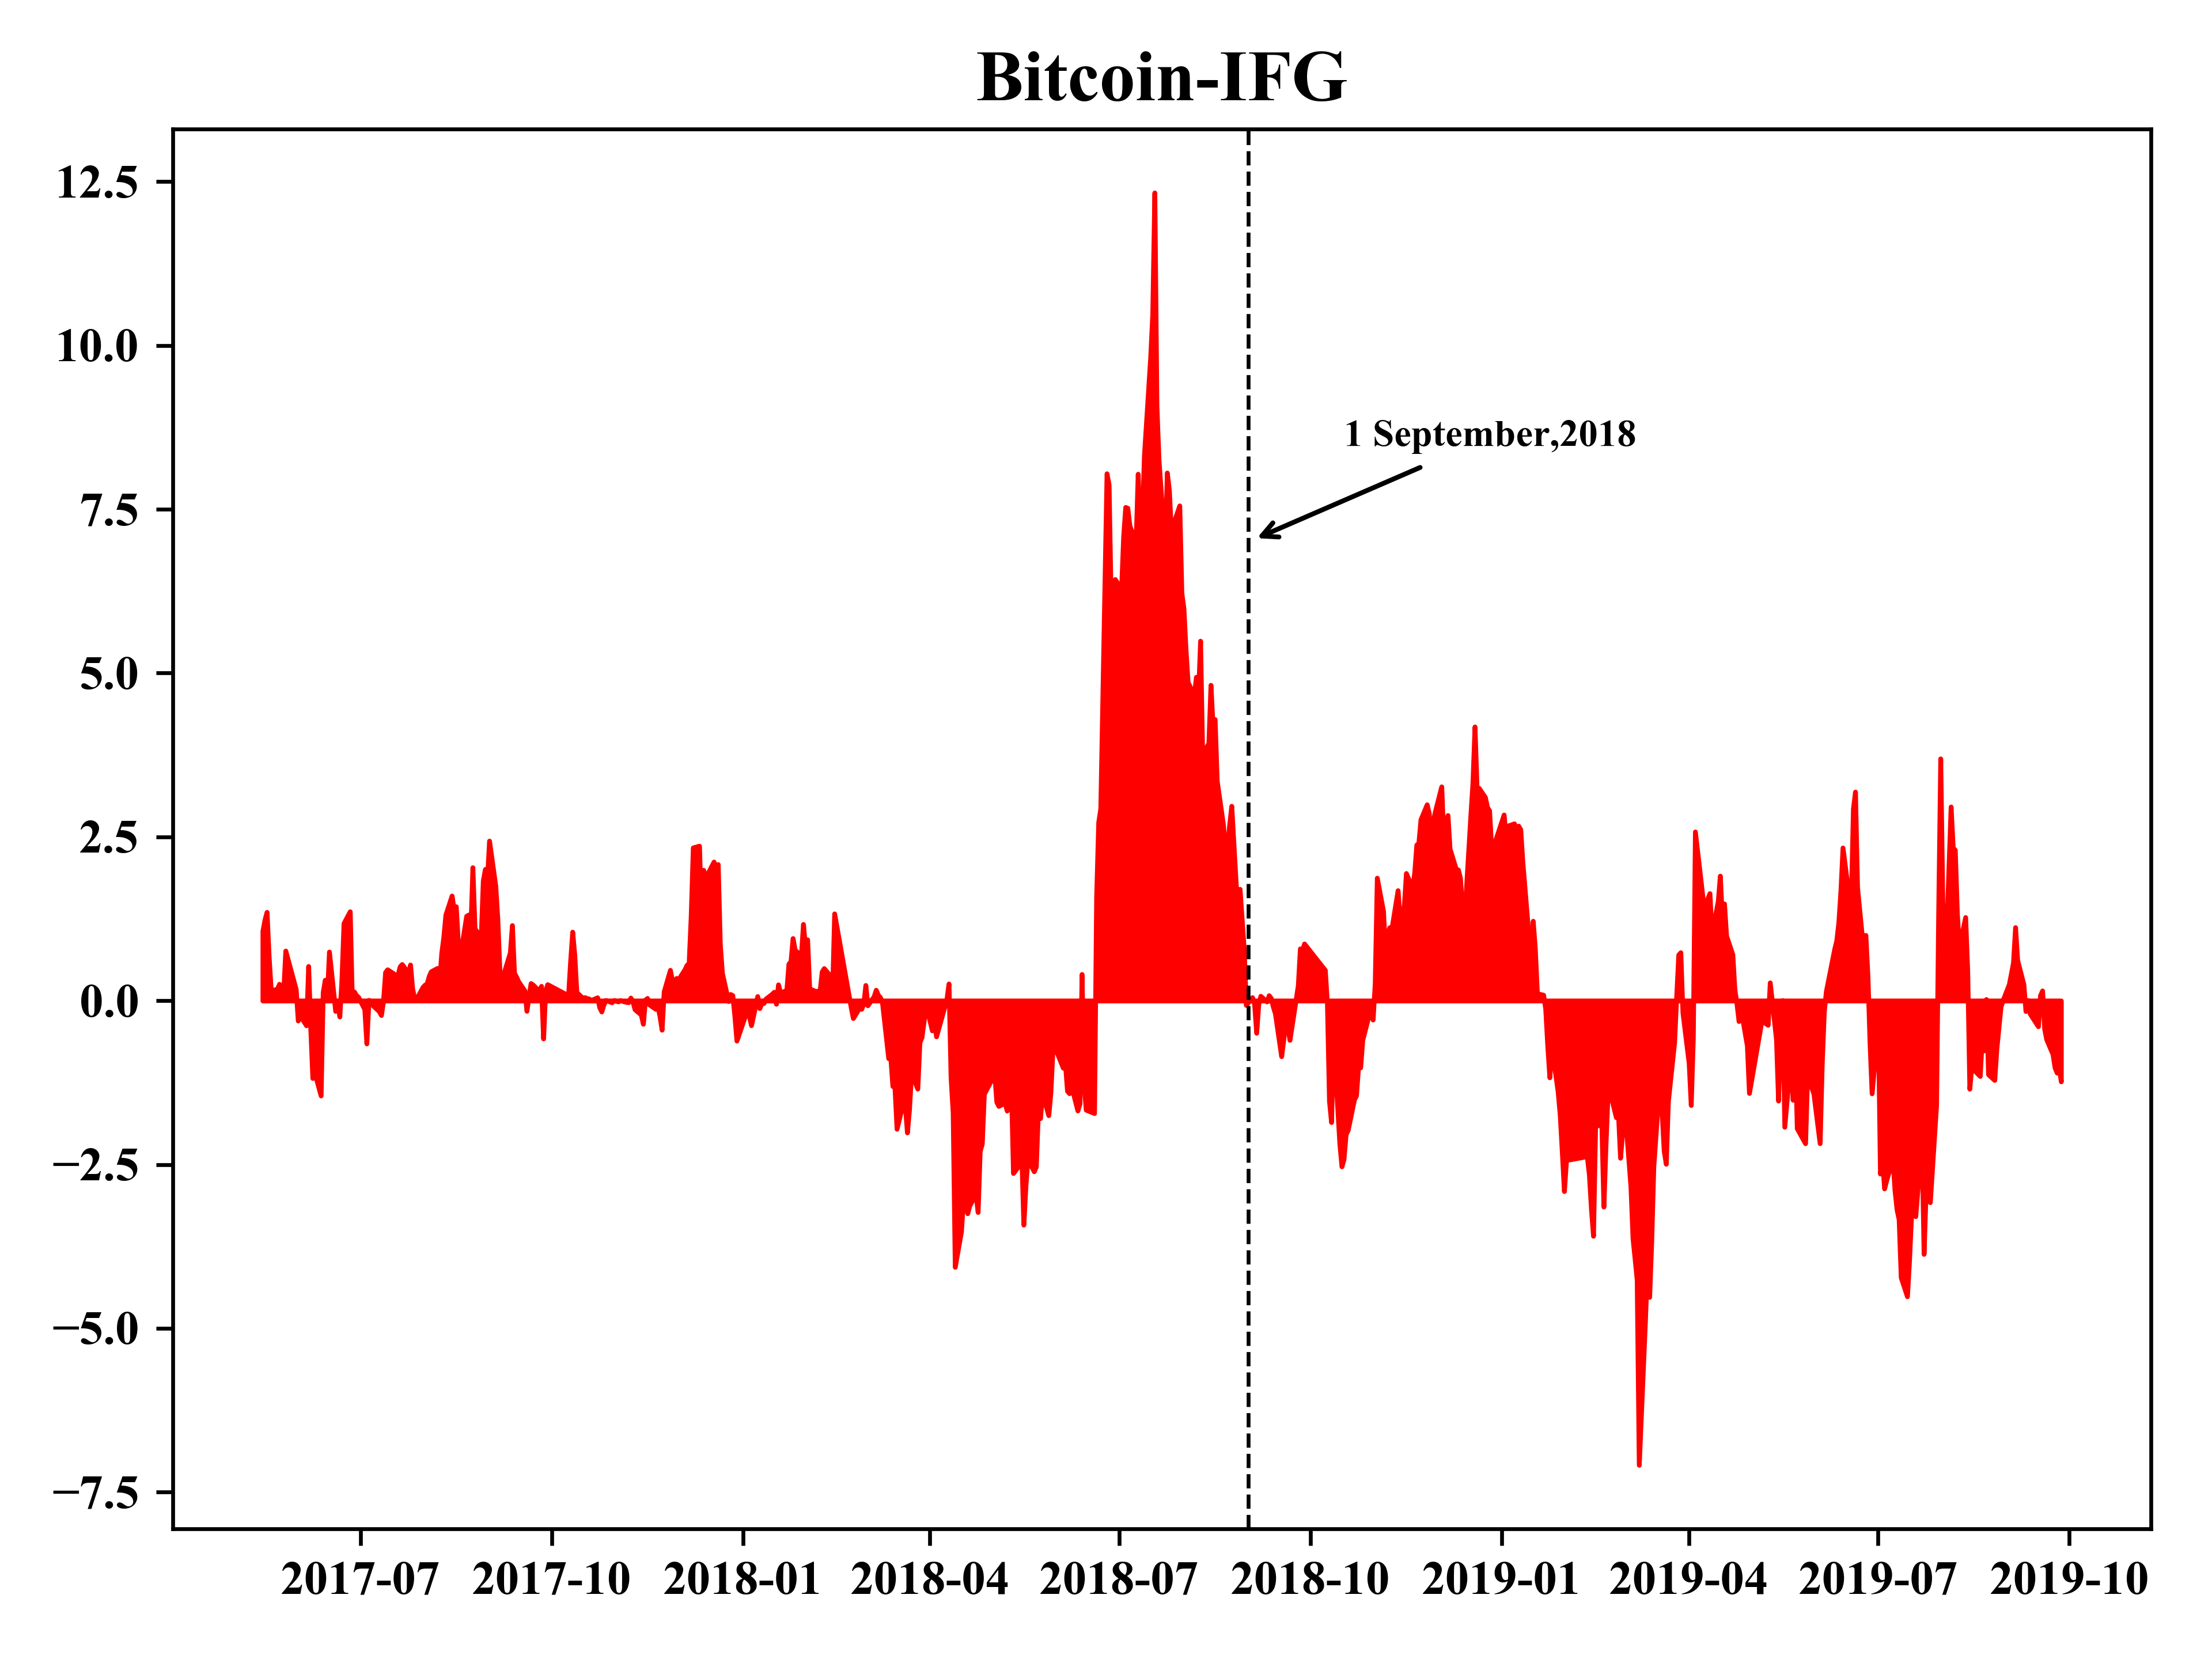
\includegraphics[width=0.45\textwidth]{IFG-NET.png}}
	
	
	\subfigure[Correlation of ISG]{
		\label{Gold.sub.3}
		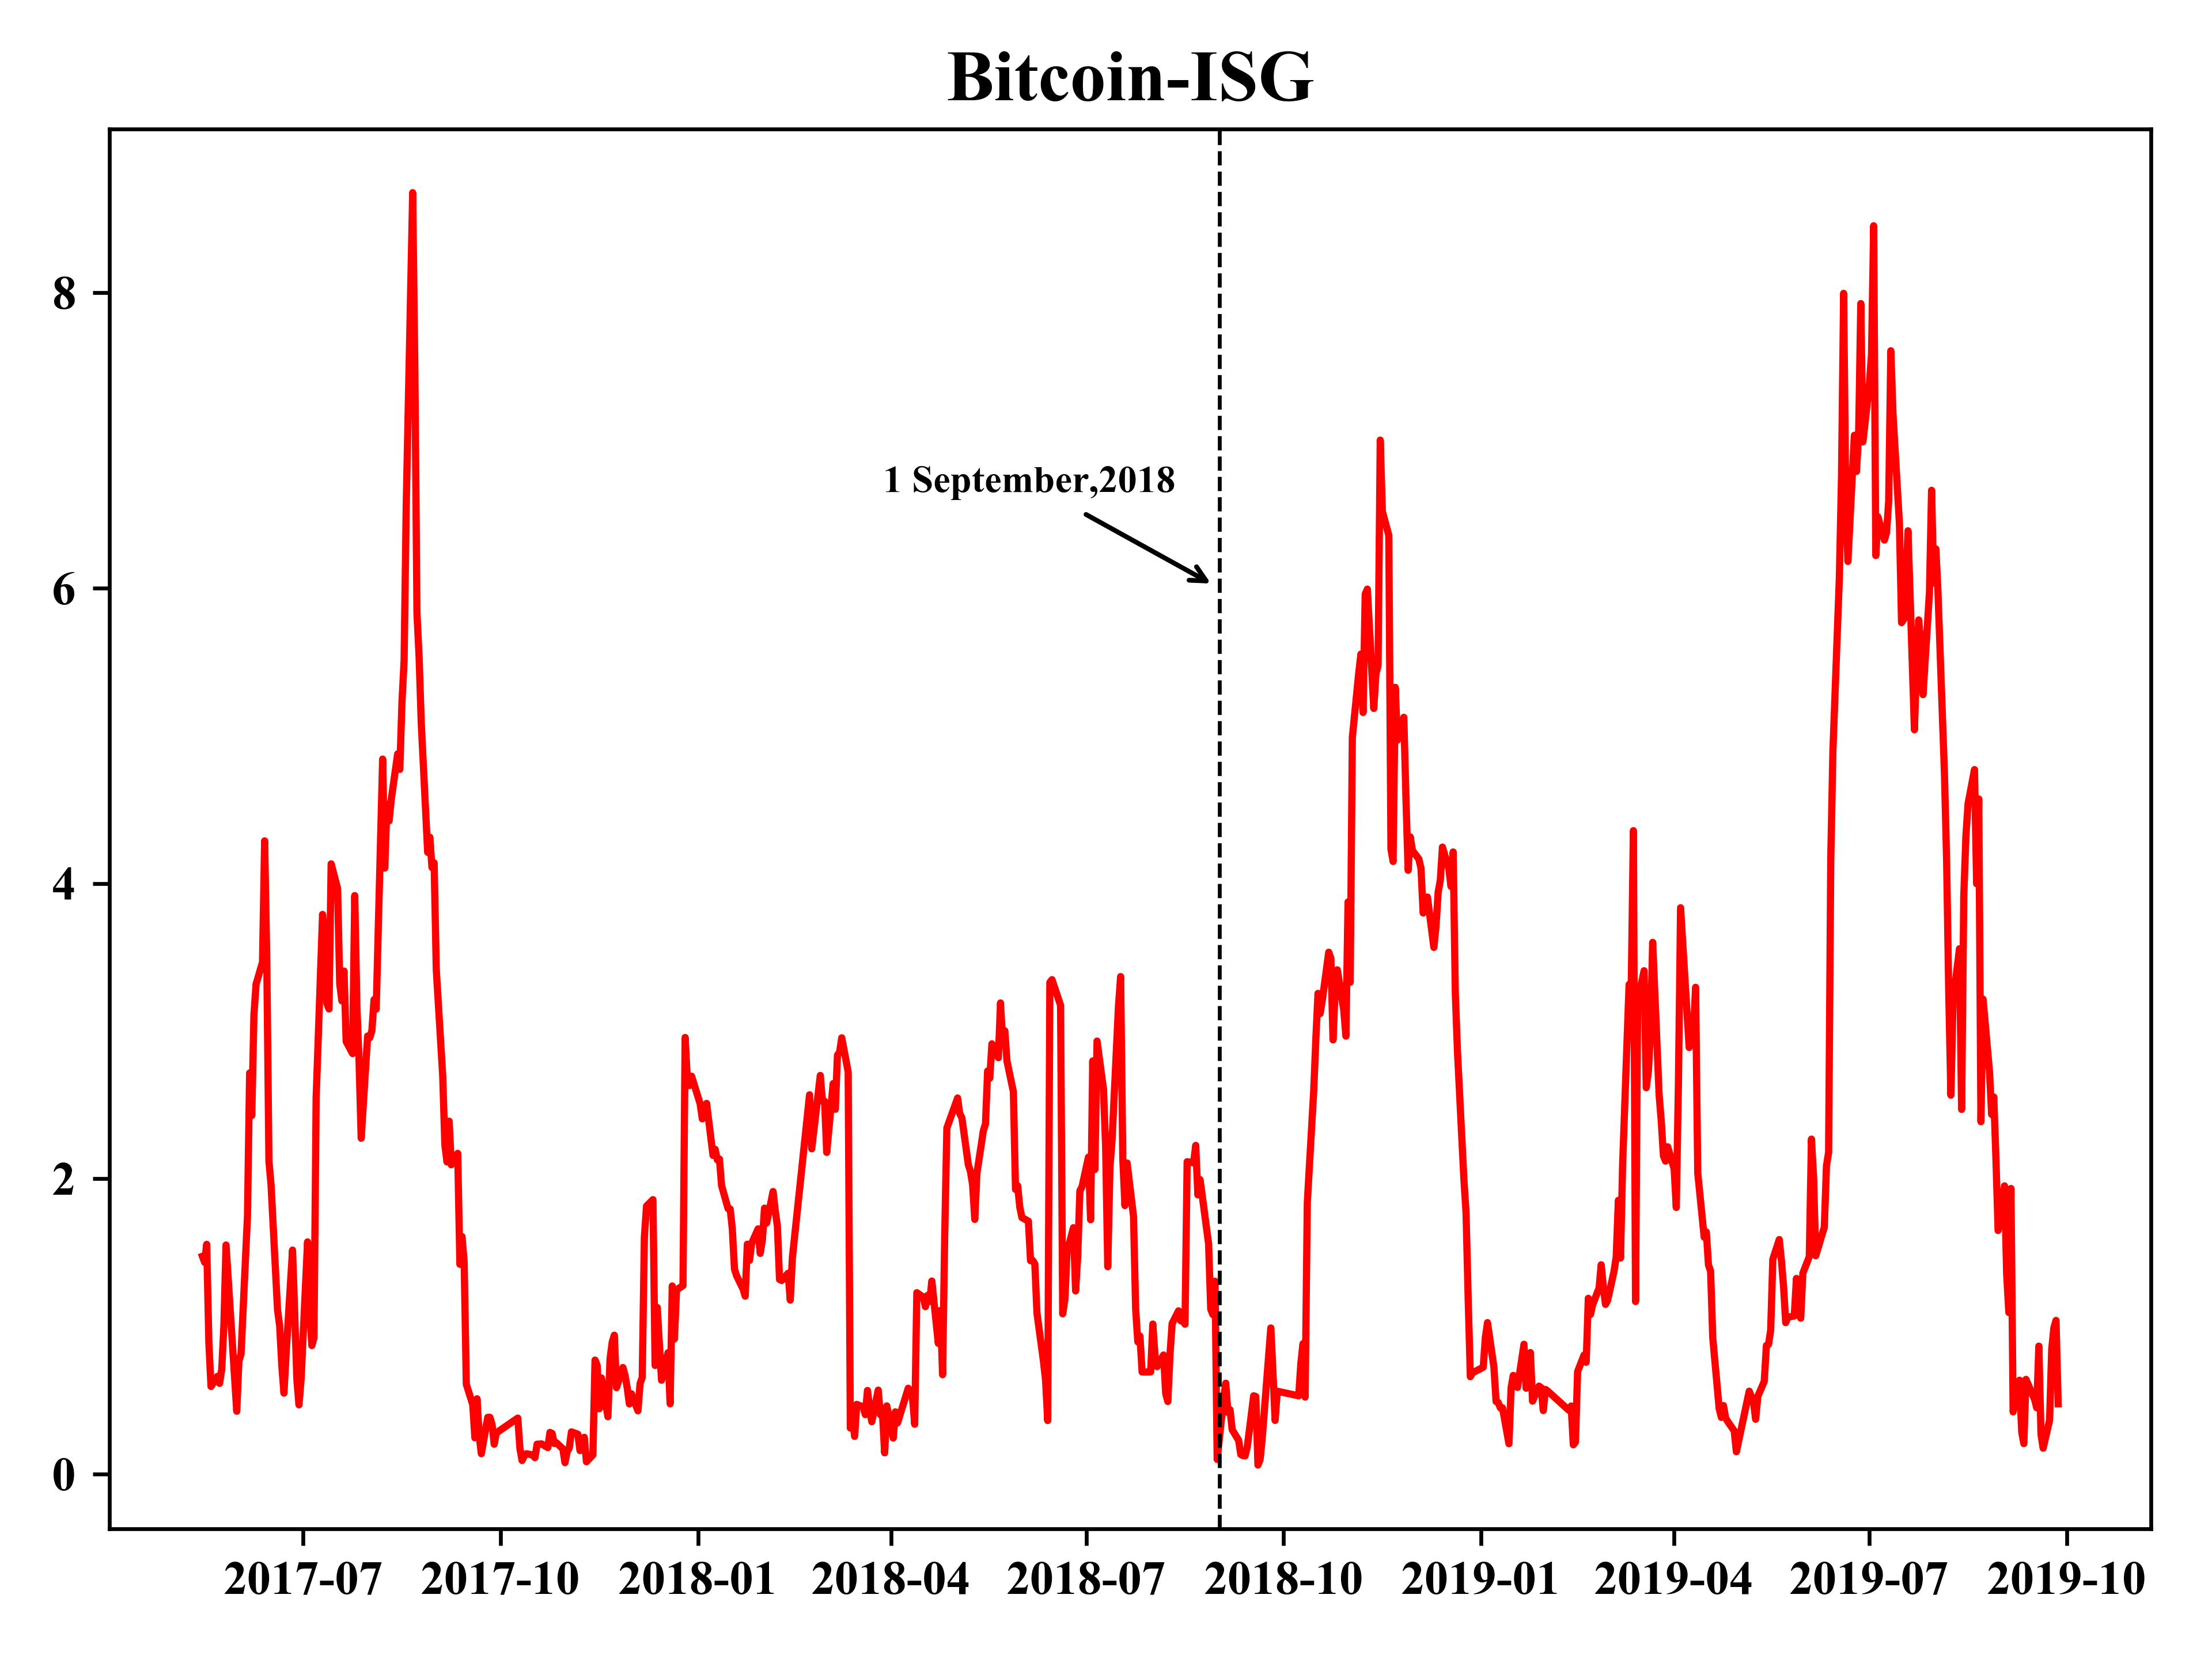
\includegraphics[width=0.45\textwidth]{ISG.png}}
	\subfigure[NPVS of ISG]{
		\label{Gold.sub.4}
		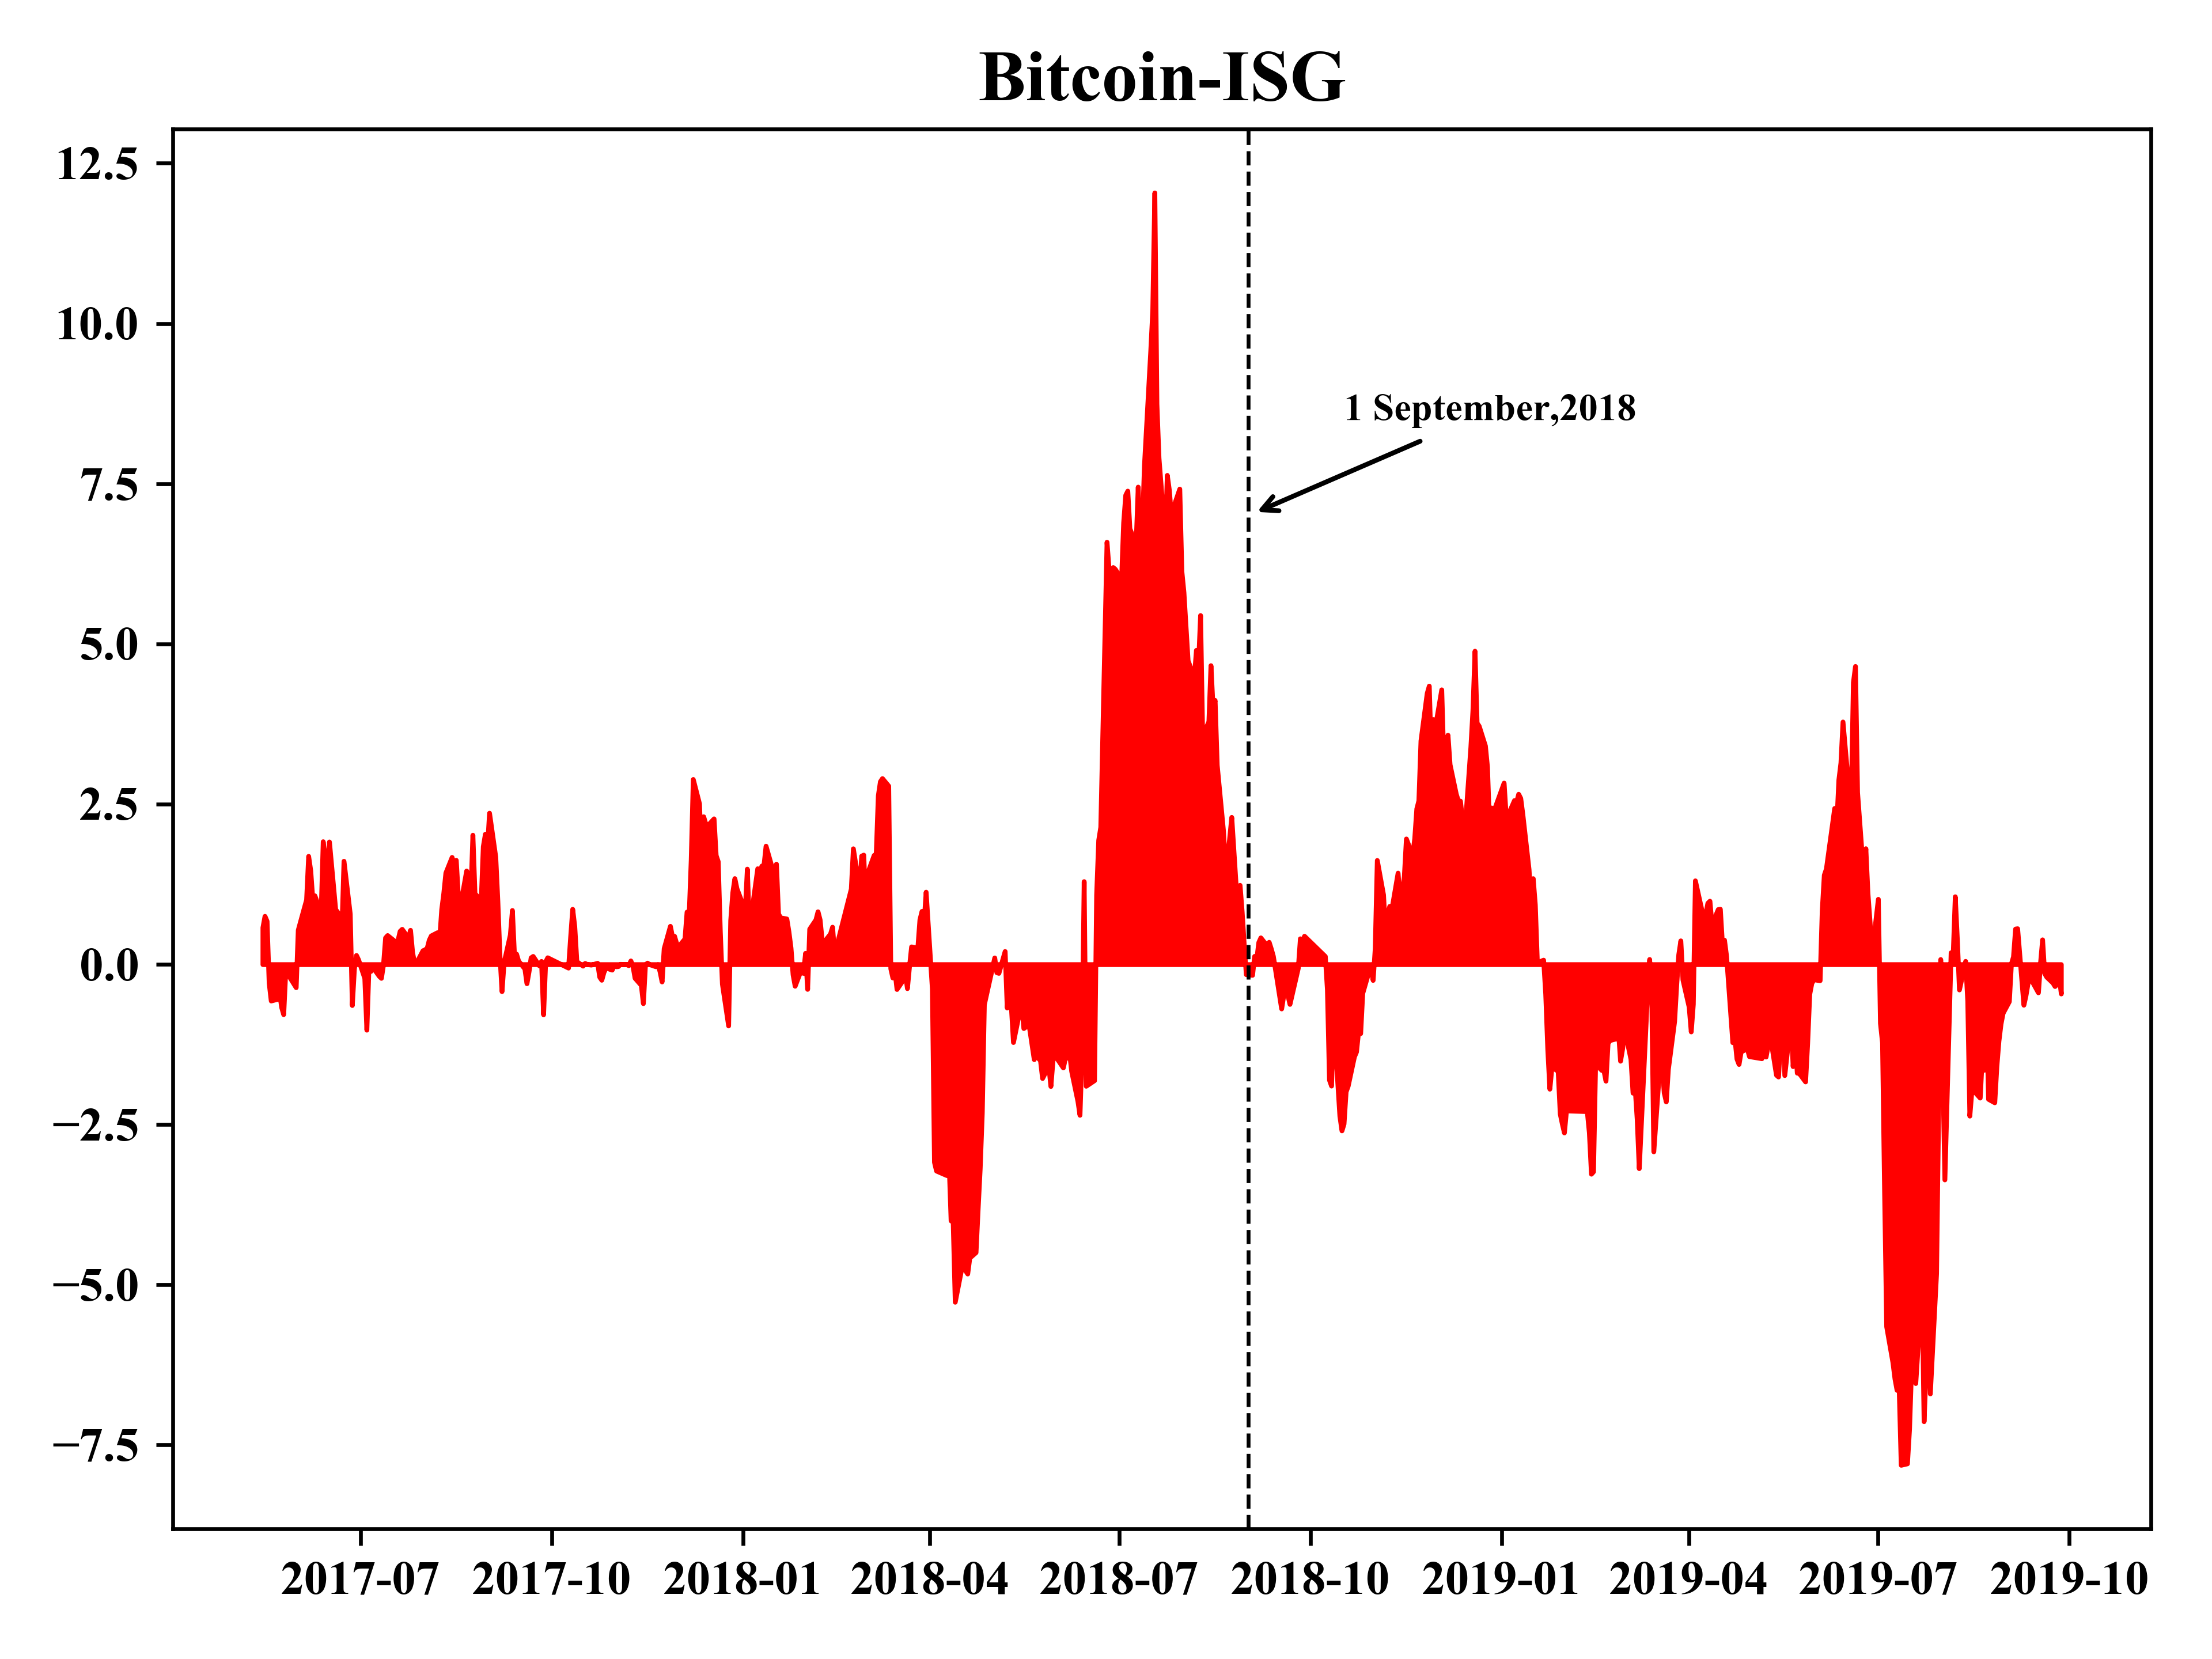
\includegraphics[width=0.45\textwidth]{ISG-NET.png}}
	
	
	\subfigure[Correlation of DFG]{
		\label{Gold.sub.5}
		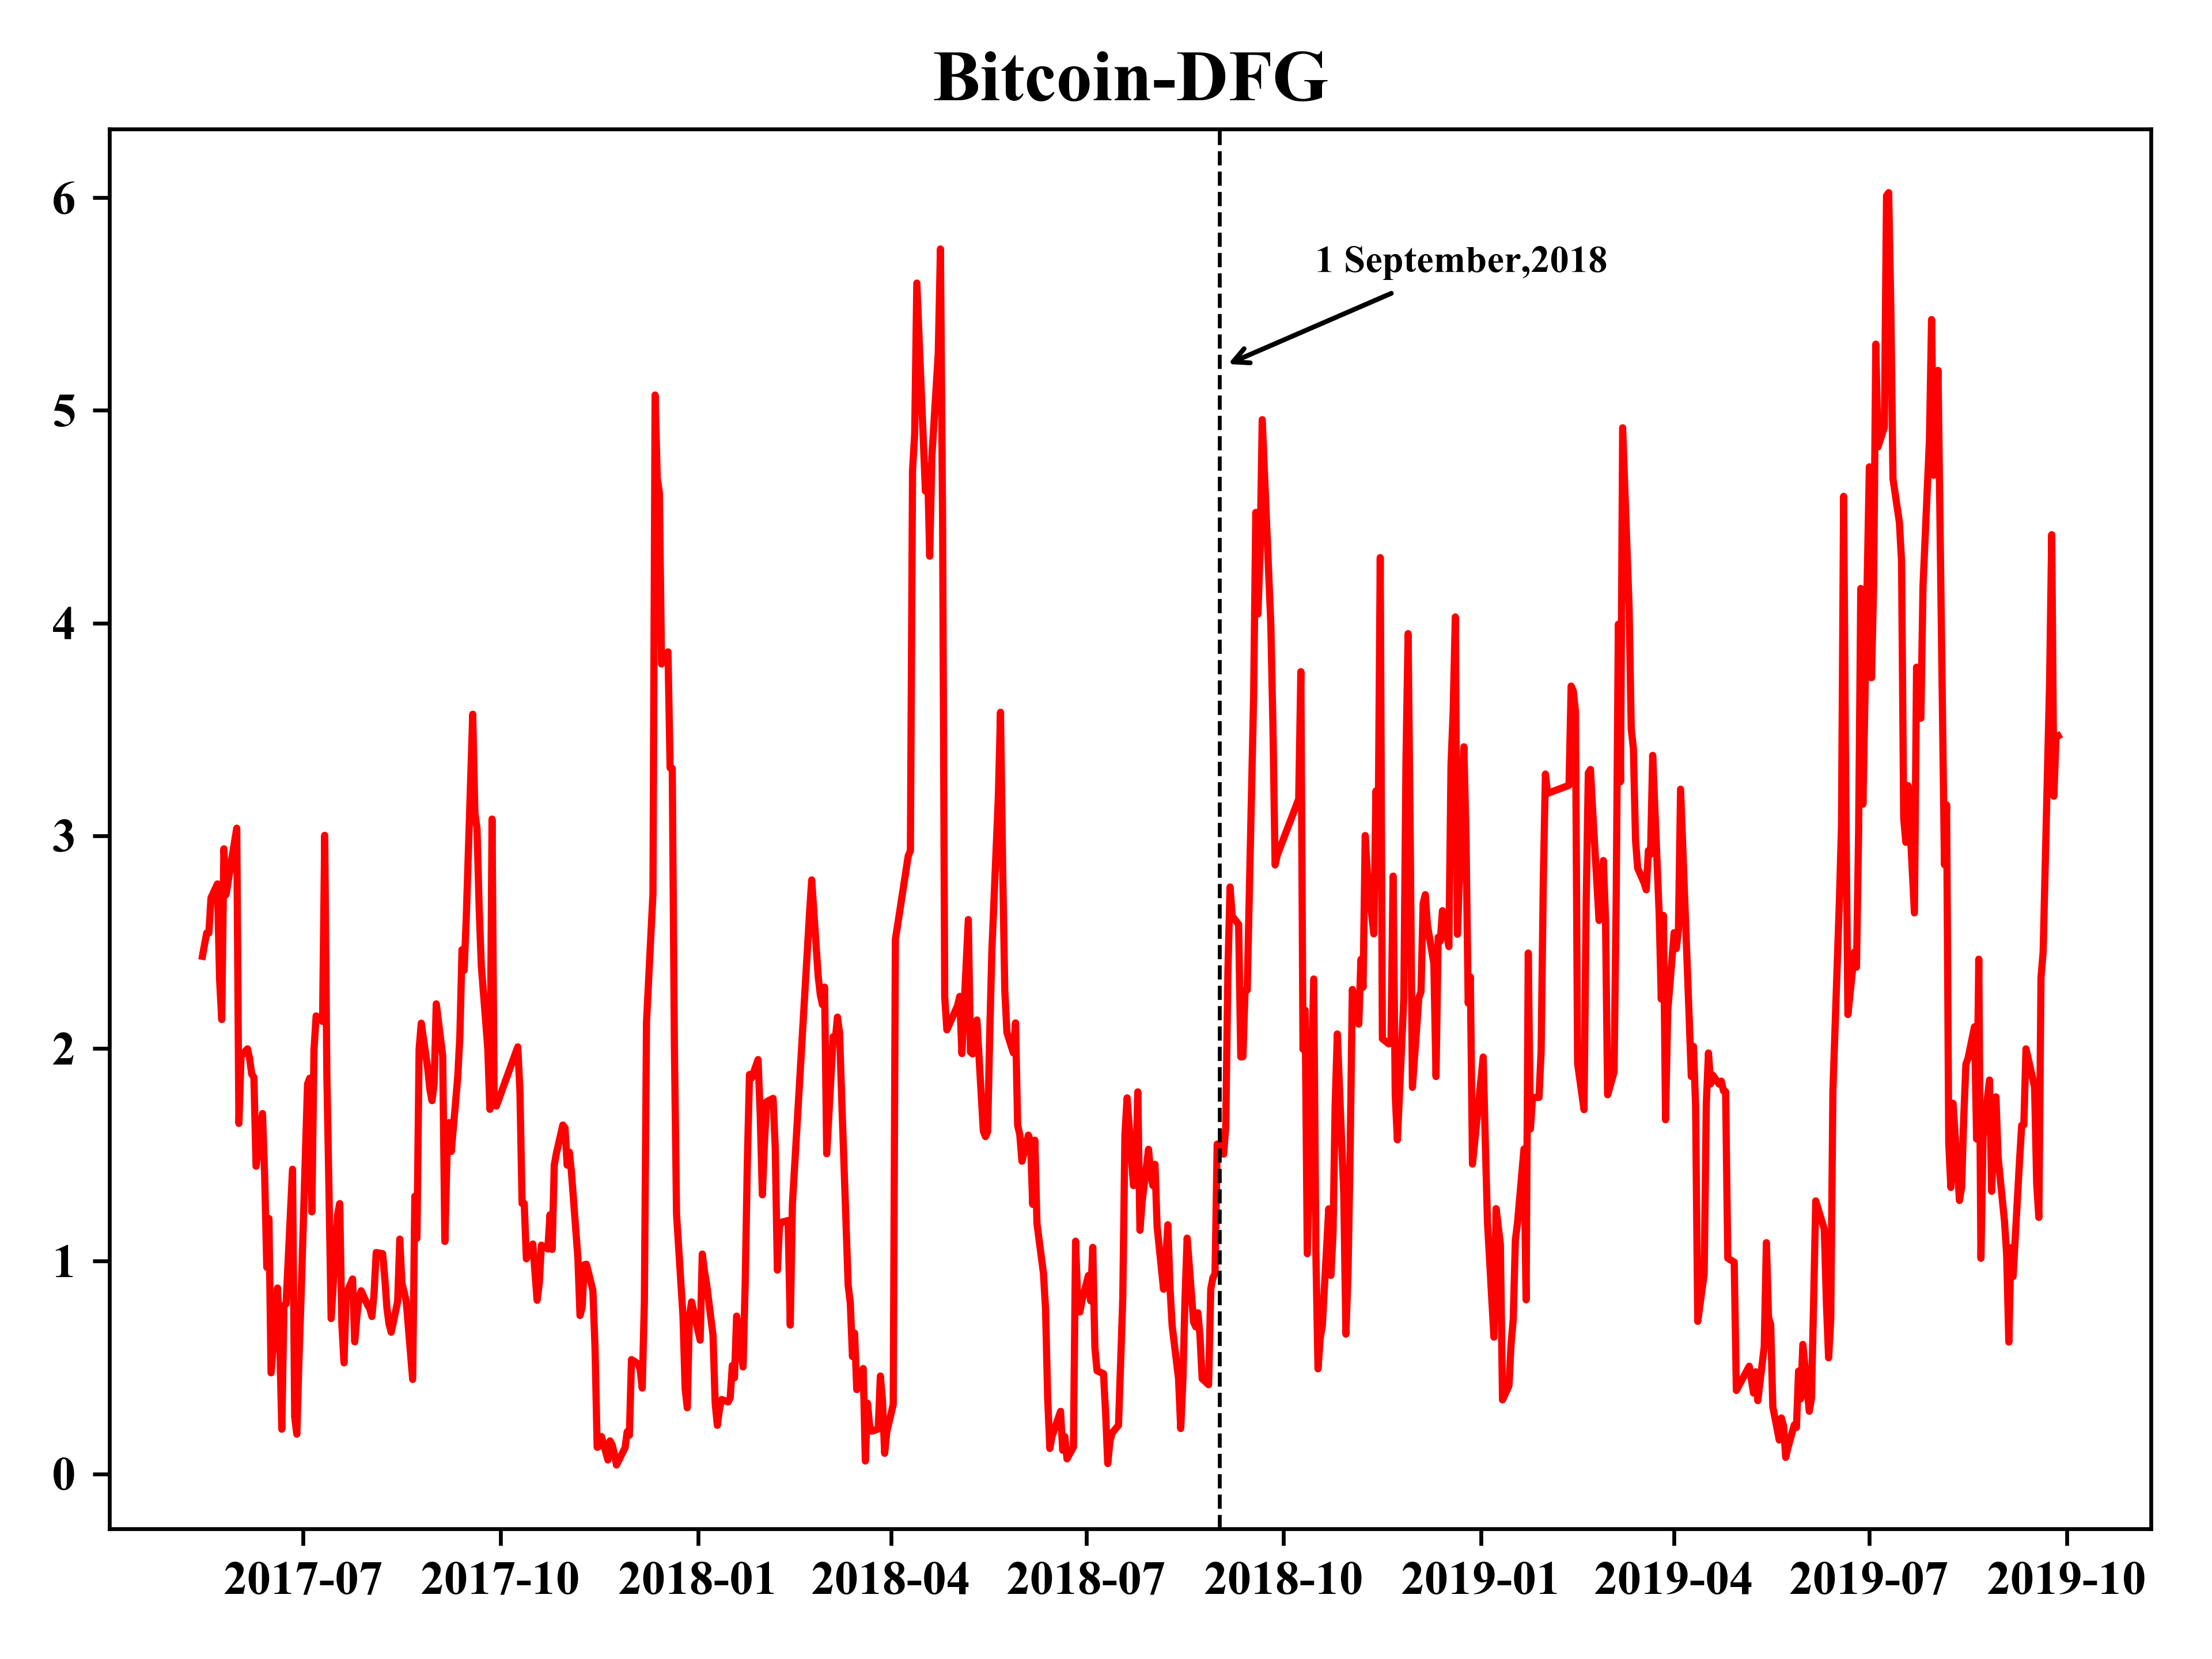
\includegraphics[width=0.45\textwidth]{DFG.png}}
	\subfigure[NPVS of DFG]{
		\label{Gold.sub.6}
		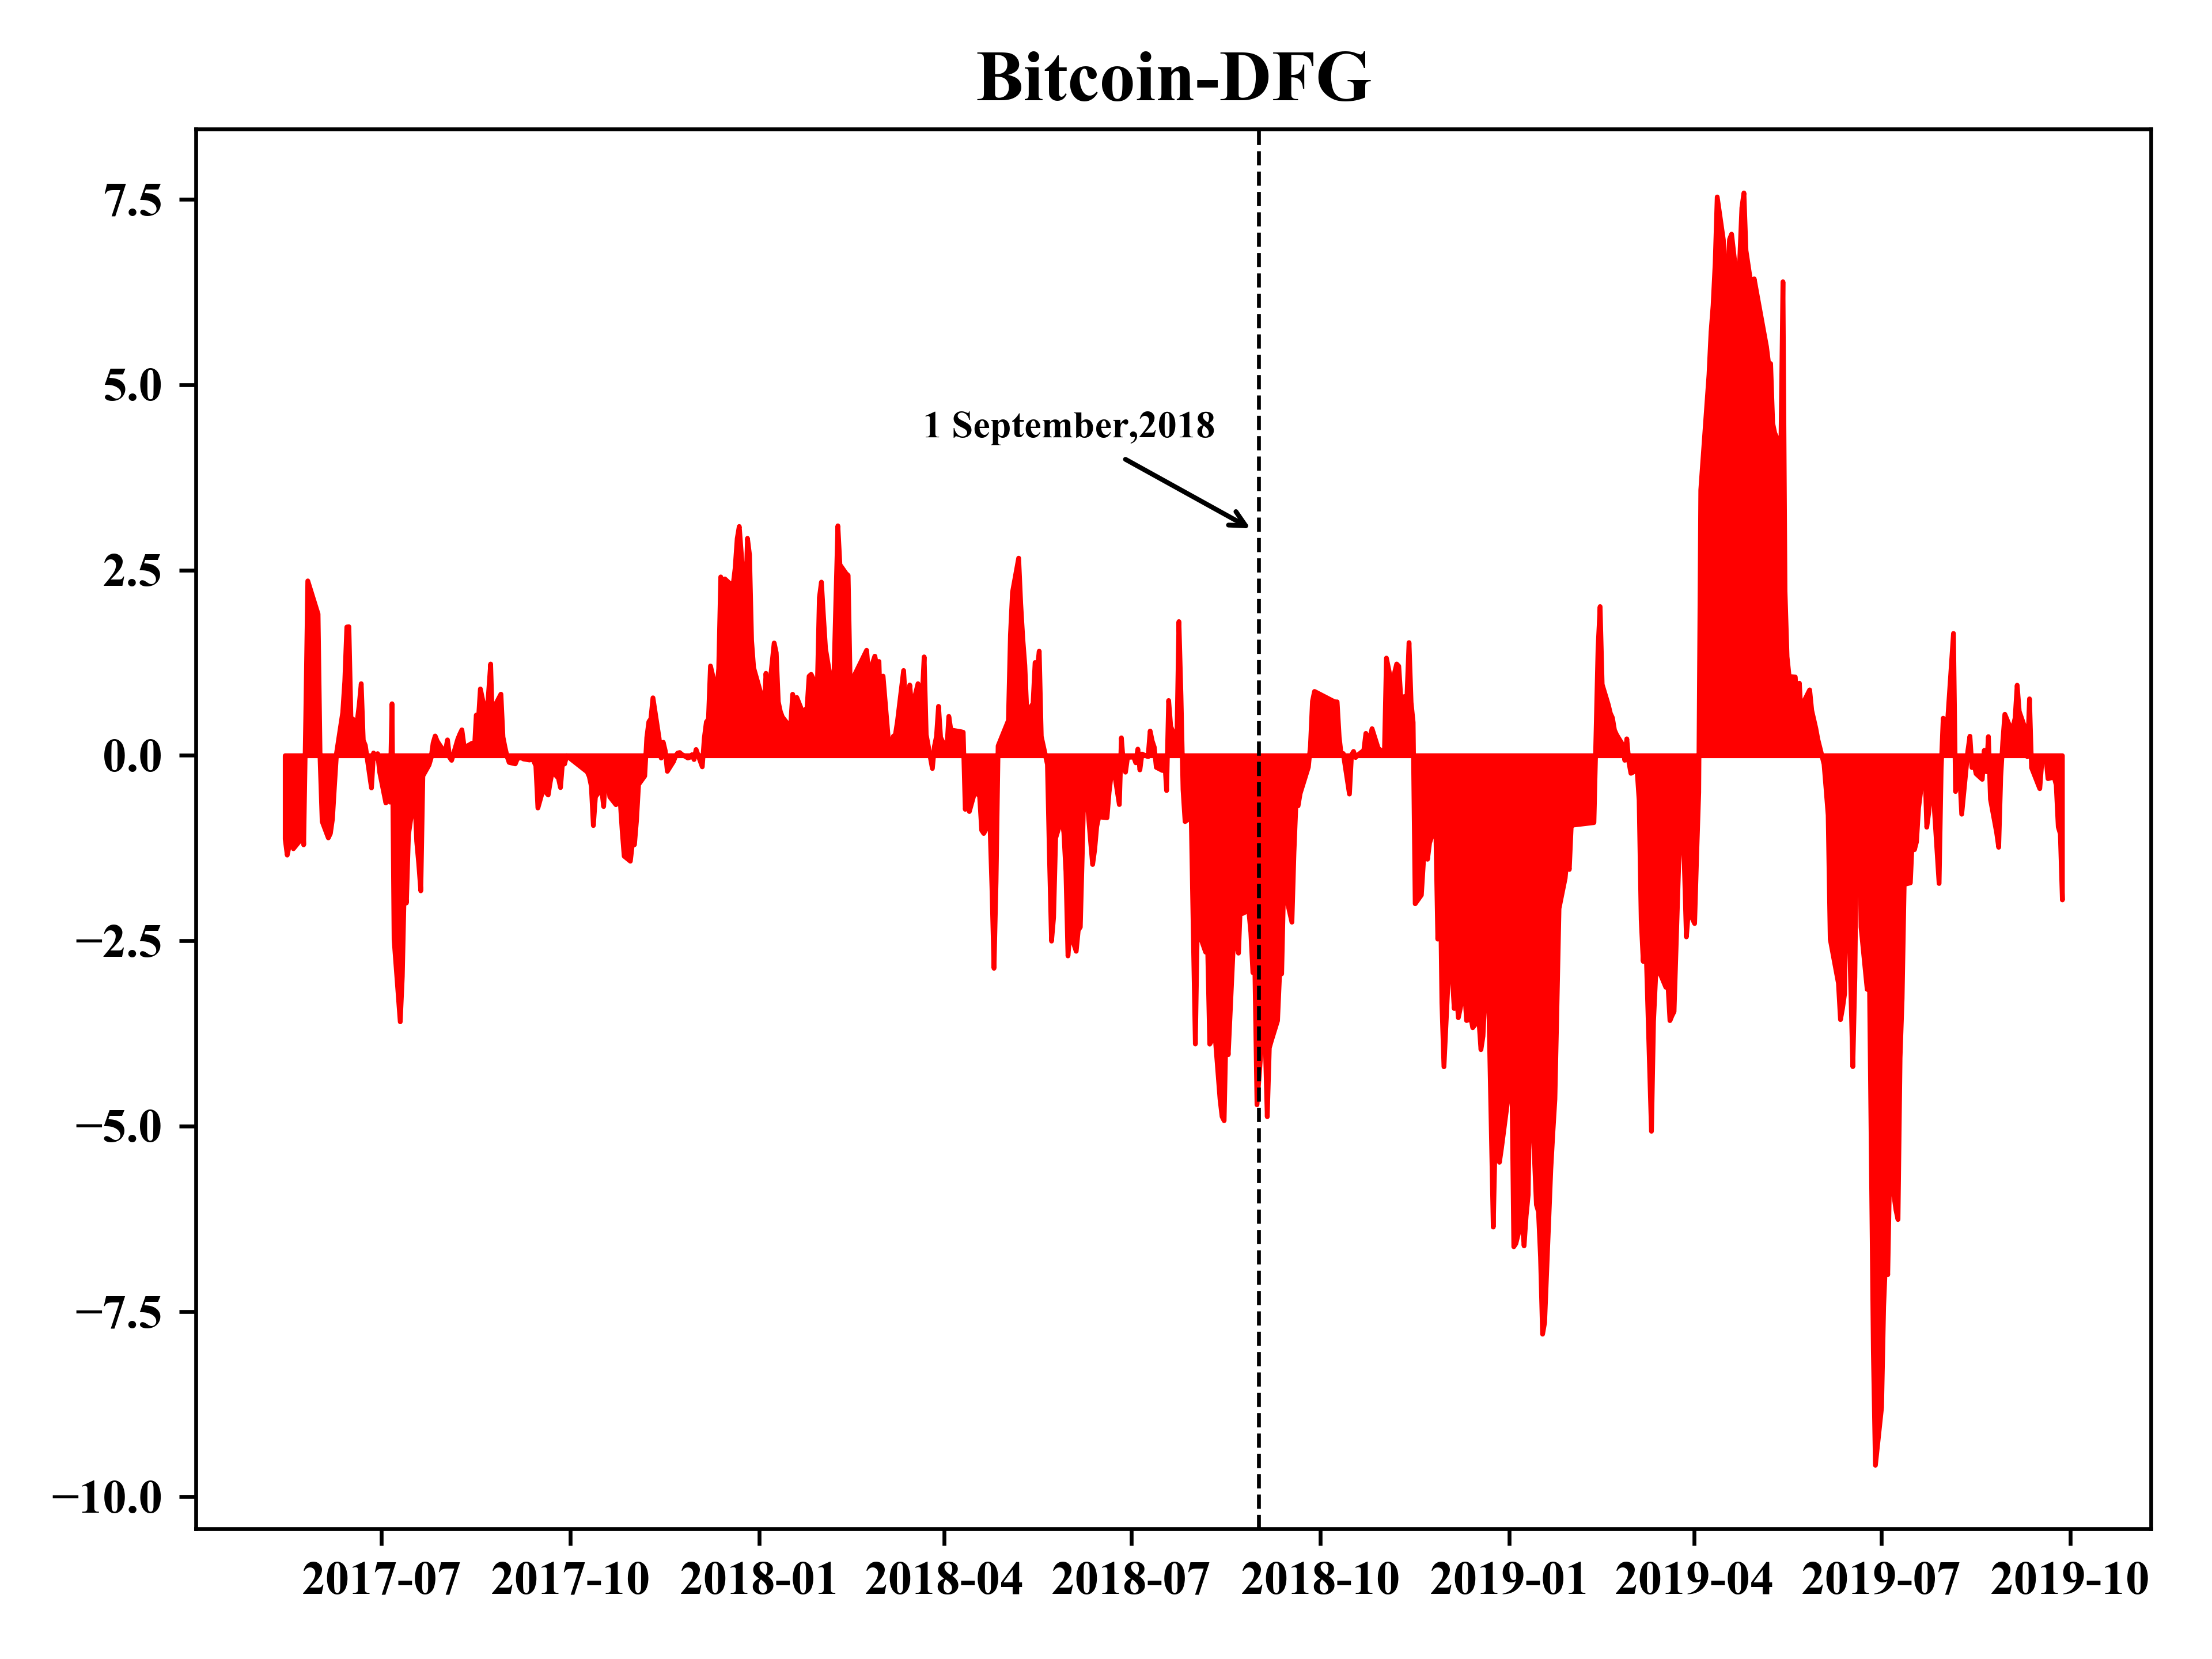
\includegraphics[width=0.45\textwidth]{DFG-NET.png}}
	
	\caption{The correlation and net pairwise volatility spillover of three golds assets}
	\label{Gold.main}
\end{figure}


Table \ref{tab4} is an overview during each period, and then we turn to elaborate the correlation and net pairwise volatility spillover in two stages. As Figure \ref{Gold.main} shows, we present three gold assets in stages. Firstly, on the whole, the correlation become to be more closed for gold assets in the second stages. Subsequently, Bitcoin has a huge contrary in two stages. (see Figure \ref{Gold.sub.1}, \ref{Gold.sub.3} and \ref{Gold.sub.5}) In the early stage, Bitcoin is more likely a volatility contributor to these gold assets. (see the left parts of Figure \ref{Gold.sub.2}, \ref{Gold.sub.4} and \ref{Gold.sub.6}) However, this become to change during the second stages. It seems that the correlation becomes to significantly emerge after the second phase. Finally, following the left part of Figure \ref{Gold.sub.5} and \ref{Gold.sub.6}, domestic future gold is a little difference between two directions in the first Stage, while the correlation fluctuates.This reveals that Bitcoin is closely related to DFG.


\begin{figure}[H]
	\centering  %图片全局居中
	\subfigure[Correlation of UFE]{
		\label{Currency.sub.1}
		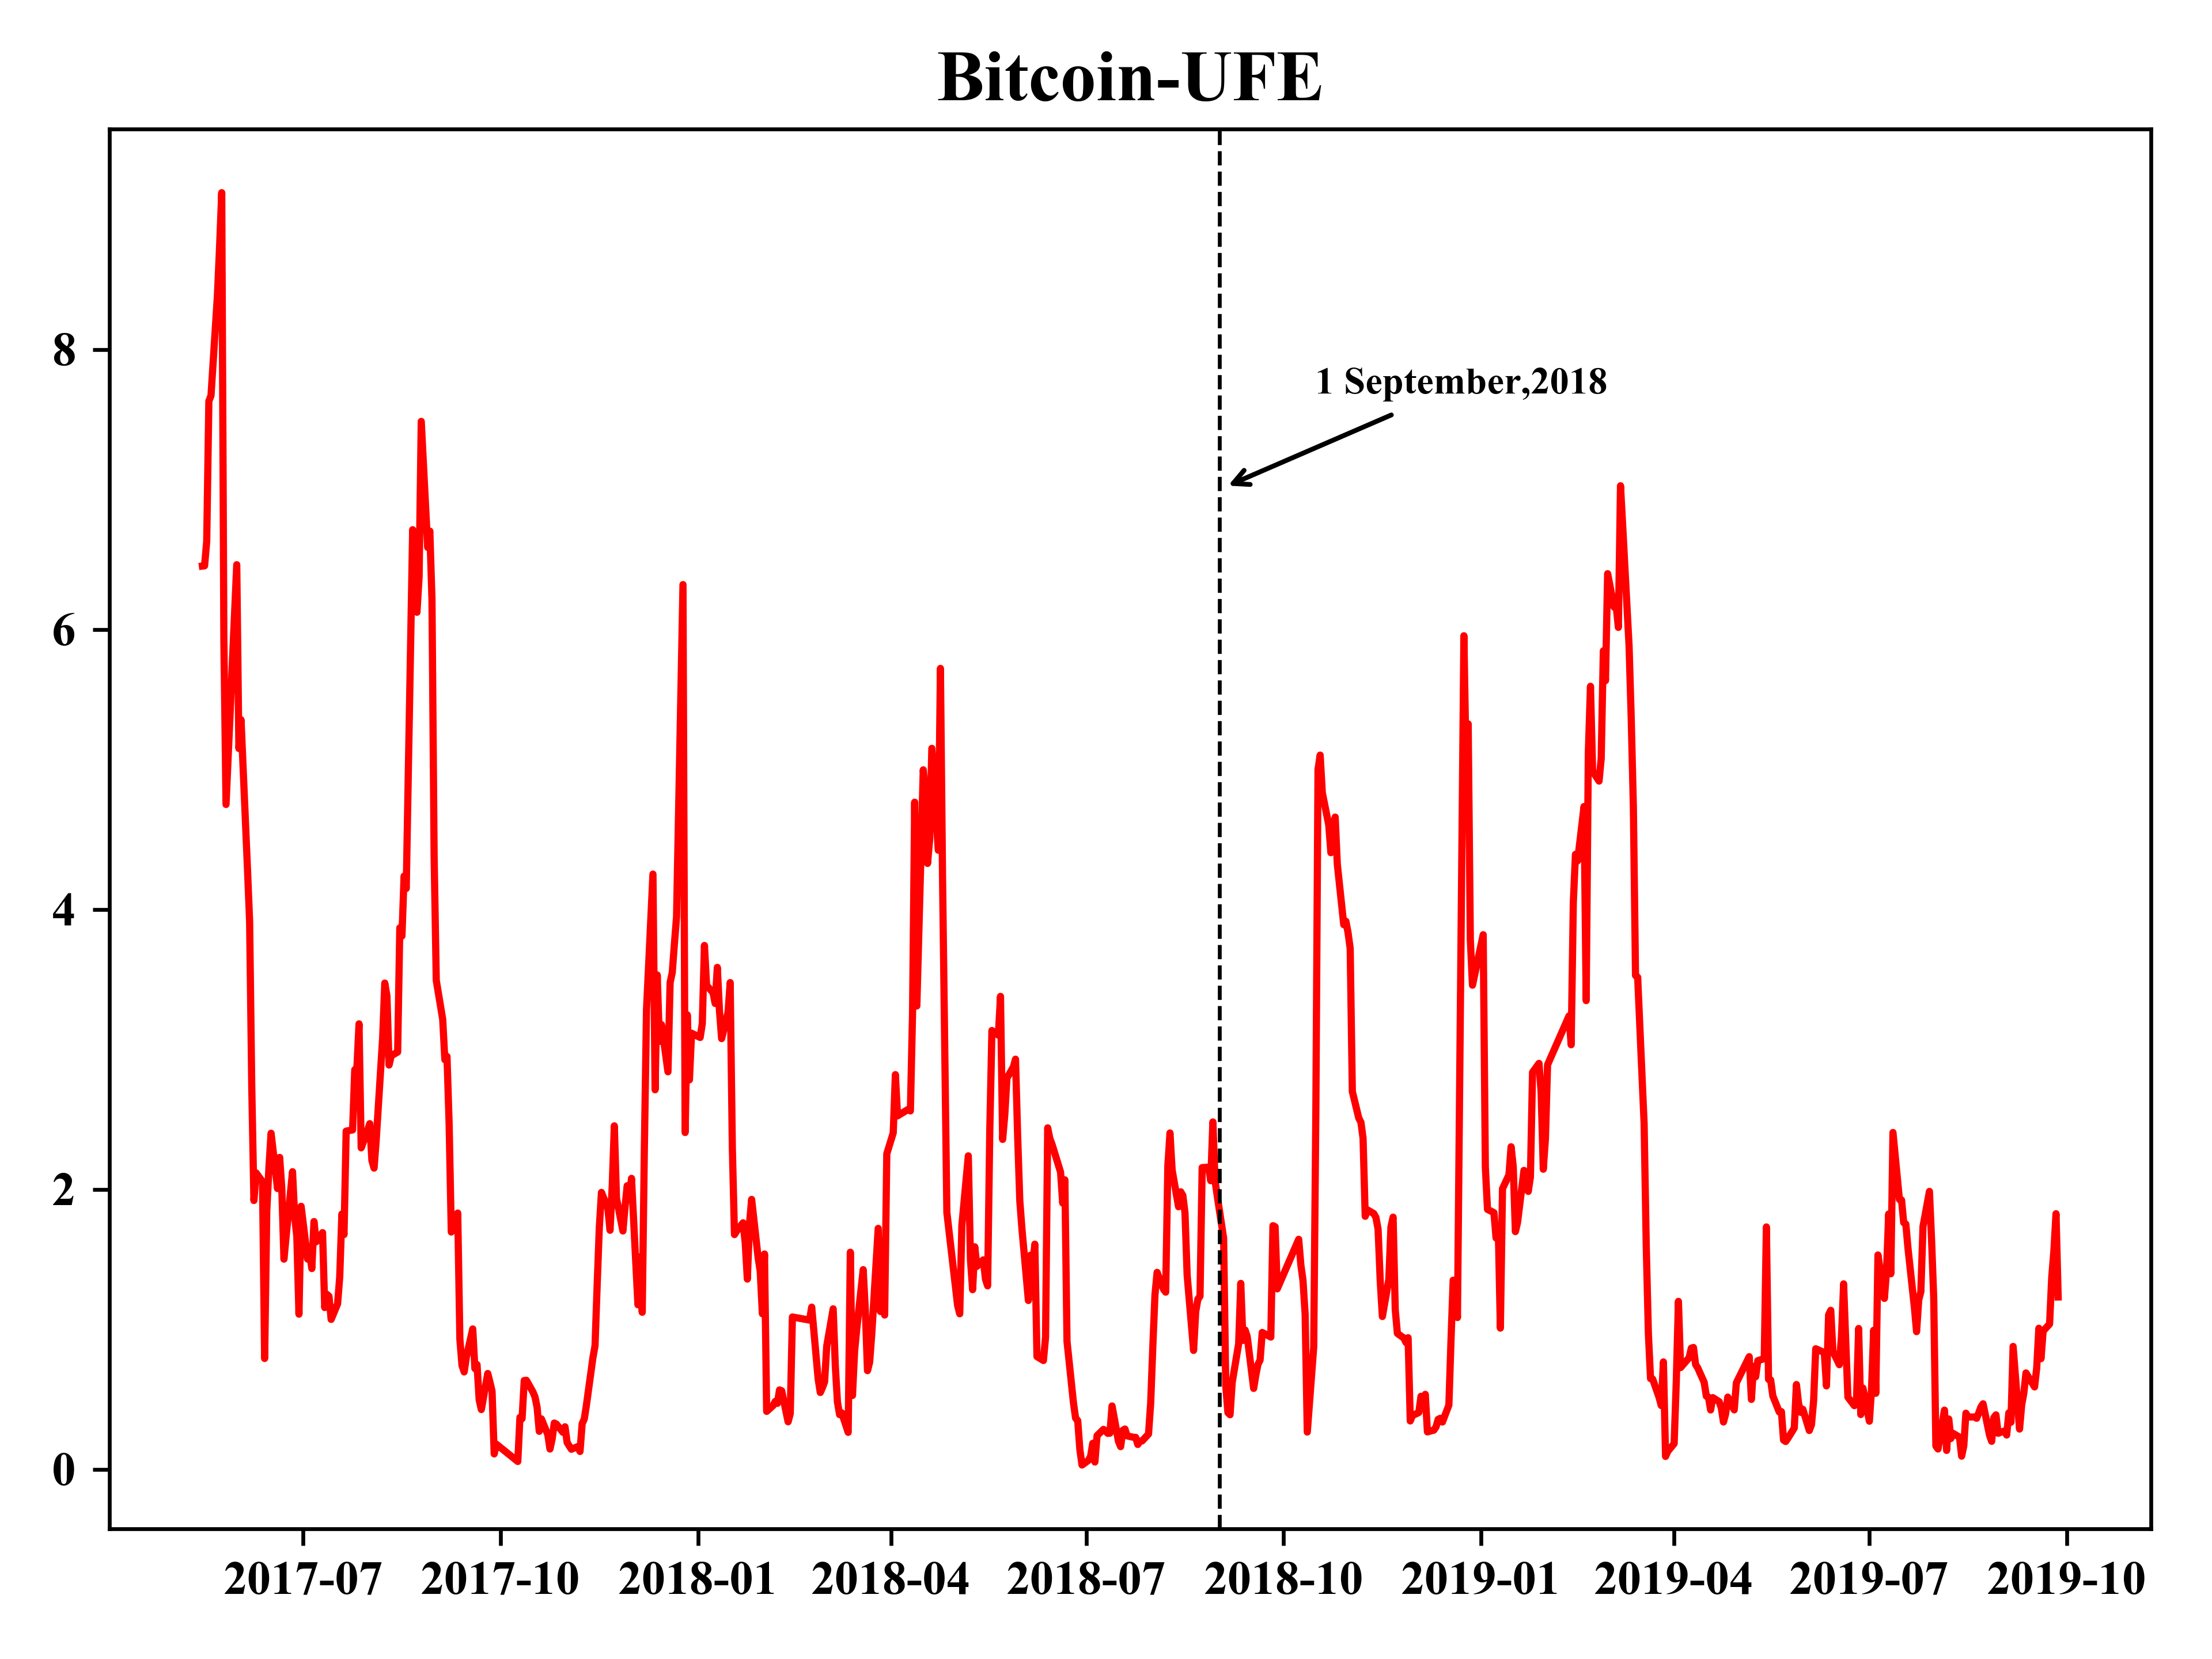
\includegraphics[width=0.45\textwidth]{UFE.png}}
	\subfigure[Correlation of UJE]{
		\label{Currency.sub.2}
		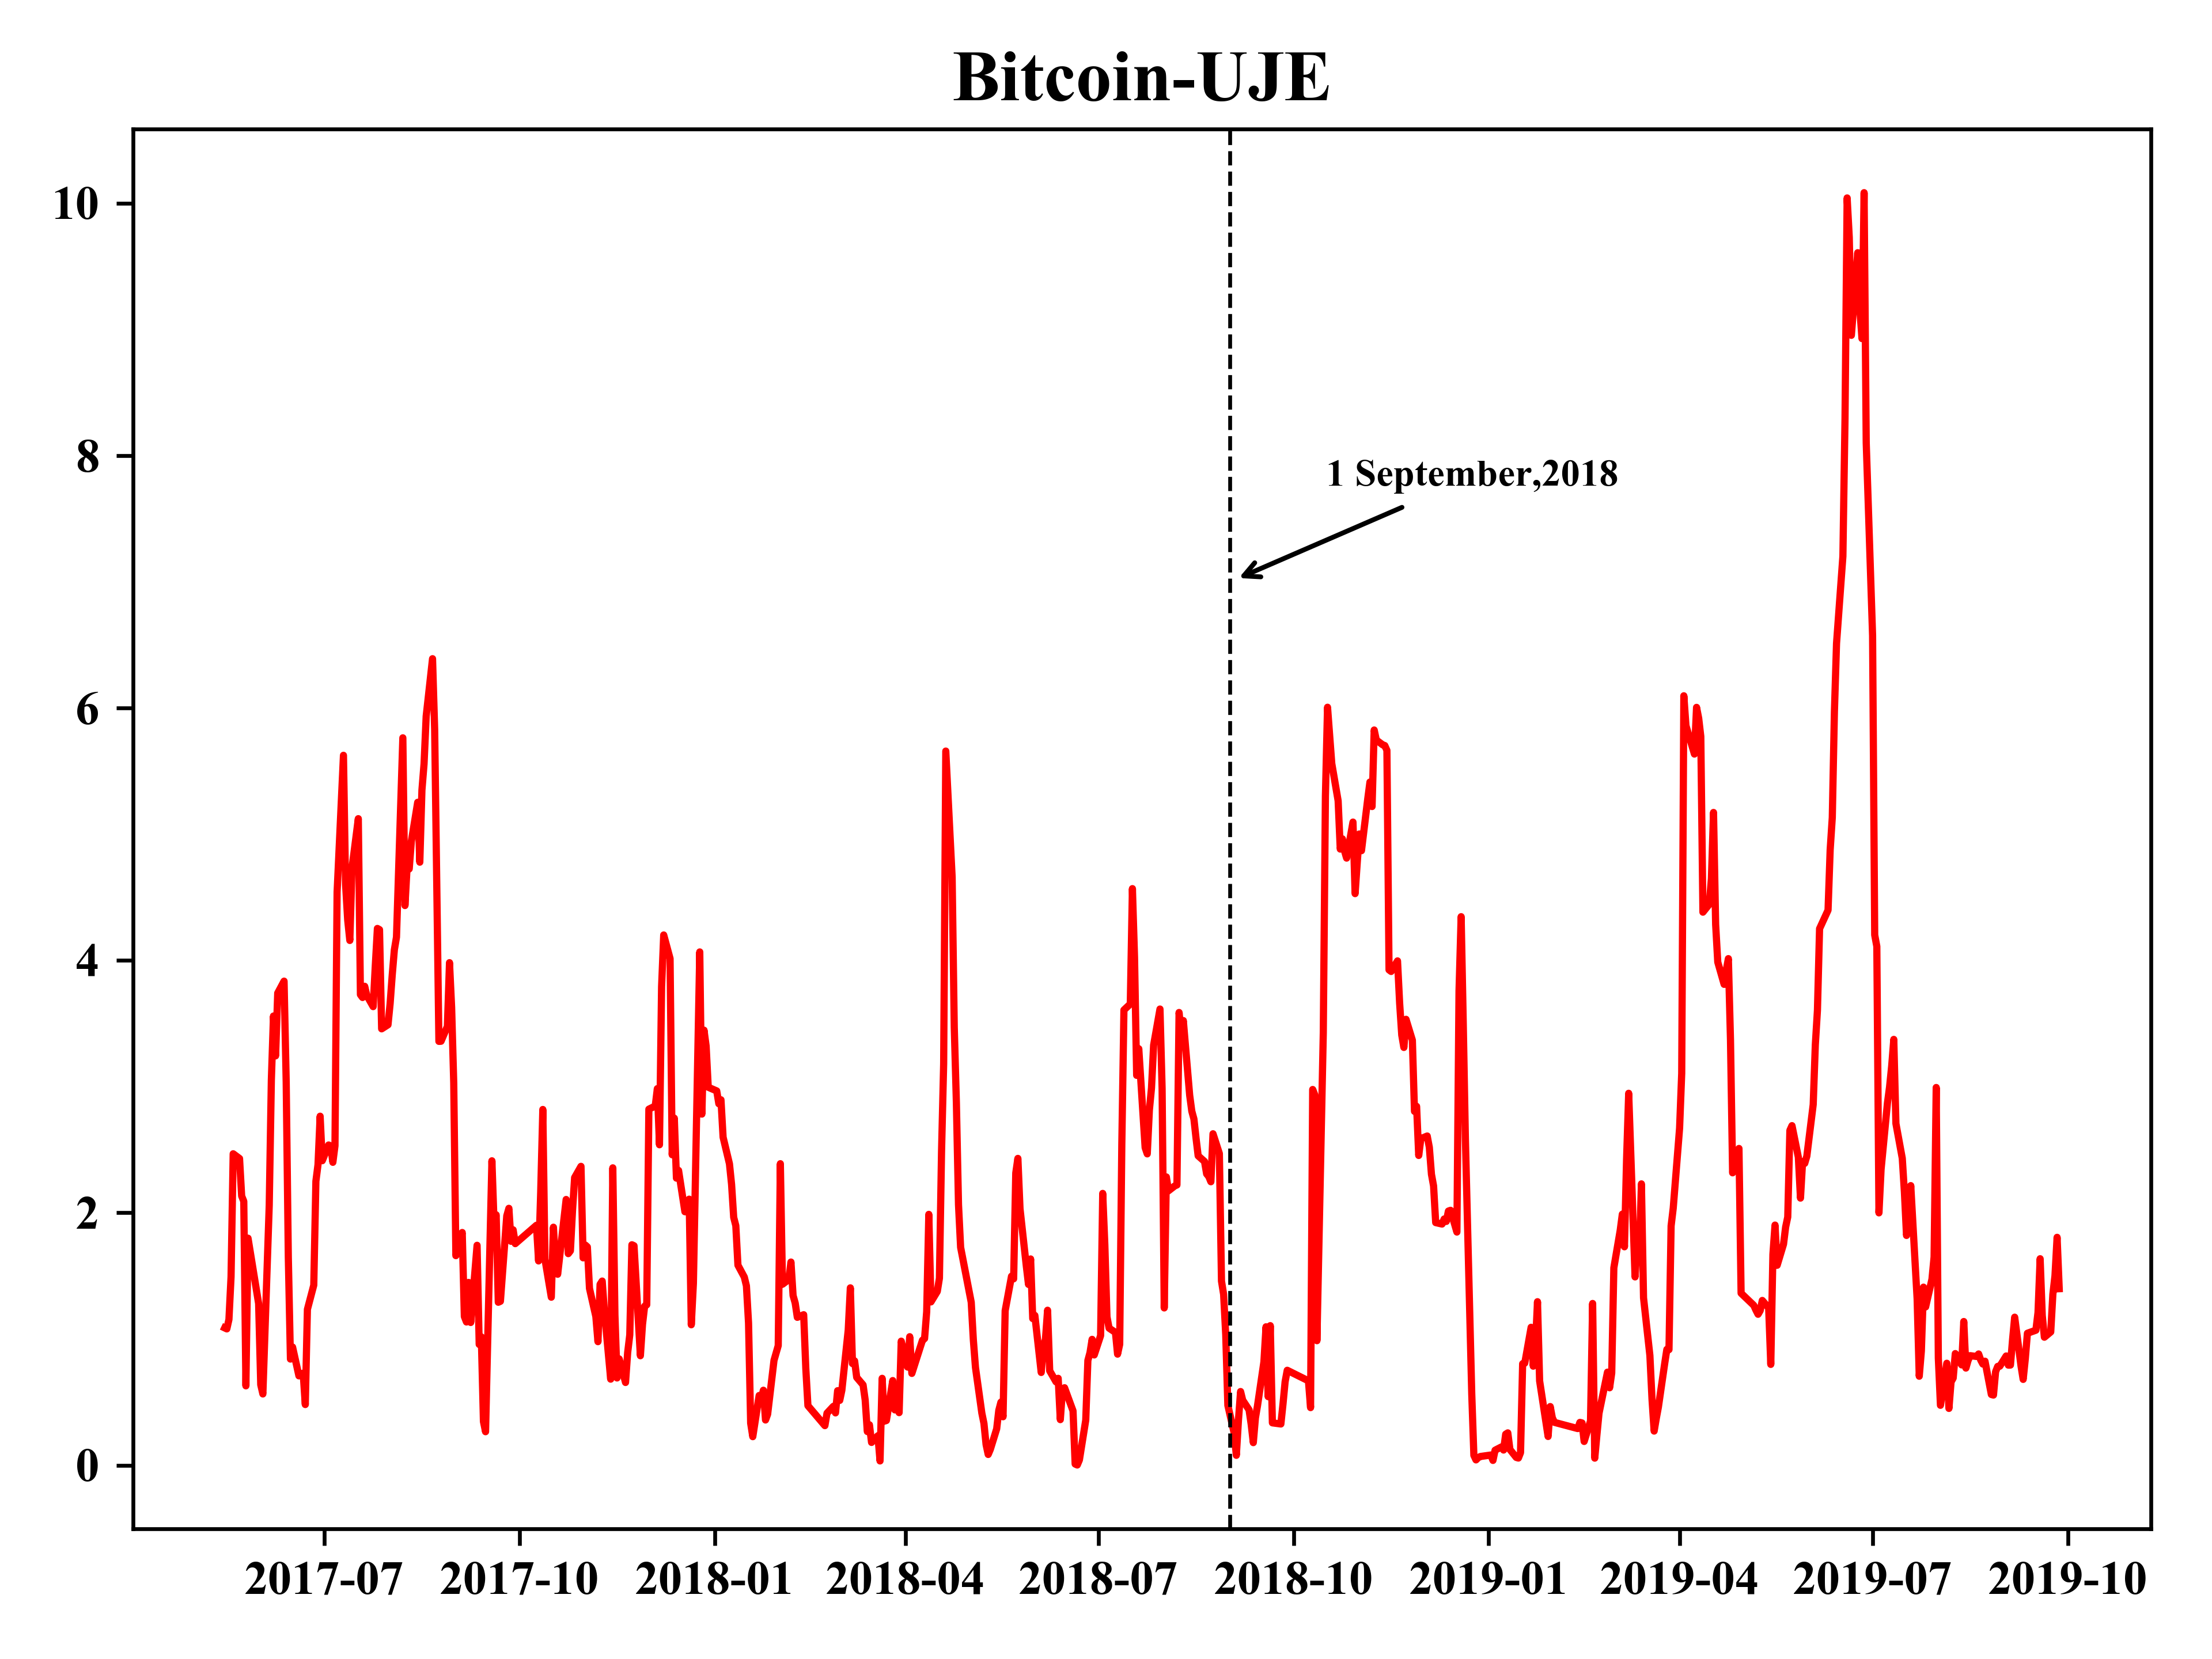
\includegraphics[width=0.45\textwidth]{UJE.png}}
	
	\caption{The correlation of the two safe-haven currencies}
	\label{Currency.main}
\end{figure}

Considering the UFE and UJE, as Figure \ref{Currency.main} shows, the two currencies increase during whole period. This corresponding phenomenon is similar to the conclusion of gold assets. Noting that the correlation of UFE become weak in recent time, which may attribute to investors' favor for gold.


In conclusion, the trend that Bitcoin is more influenced from gold assets is more likely to continue on account of the Sino-US trade dispute. This also strengths the perspective that Bitcoin has become a global safe haven asset. Additionally, the two currencies' effect to Bitcoin is replaced by gold assets, which may reveal that international investors are prefer gold asset (in particular, future gold) due to the uncertainty in the world economy. Finally, these figures also indicate that the connectednesses do not become related until the second stage, which may reveal that there are different driving factors in two stages. And we will analyze this phenomenon with Granger-Cause analysis. 

\subsubsection{Driving China' financial market opening up}
For stock market, SH300 shows a higher connectedness among these main capital markets all over the world. The volatility ratio increases from 1.32\% to 23.13\% for ``To'' direction and from 1.62\% to 5.81\% for another direction, respectively. At least two reasons can explain this phenomenon. Firstly, SH300 reflects China' market expectations. Hence, every shock of economics propagates to Bitcoin market in that Bitcoin has being becoming the safe haven asset.  Secondly, the imbalance increase of two directions may reveal that volatility of Bitcoin is much easier to influence SH300 because Bitcoin is an international asset. Therefore, it is conceivable that Bitcoin may drive (in disguised form) China's financial market to open in case the association between Bitcoin and SH300 continues to increase, which should be attached importance to.

\begin{figure}[H]
	\centering  %图片全局居中
	
	\subfigure[Correlation of SH300]{
		\label{SH300.sub.1}
		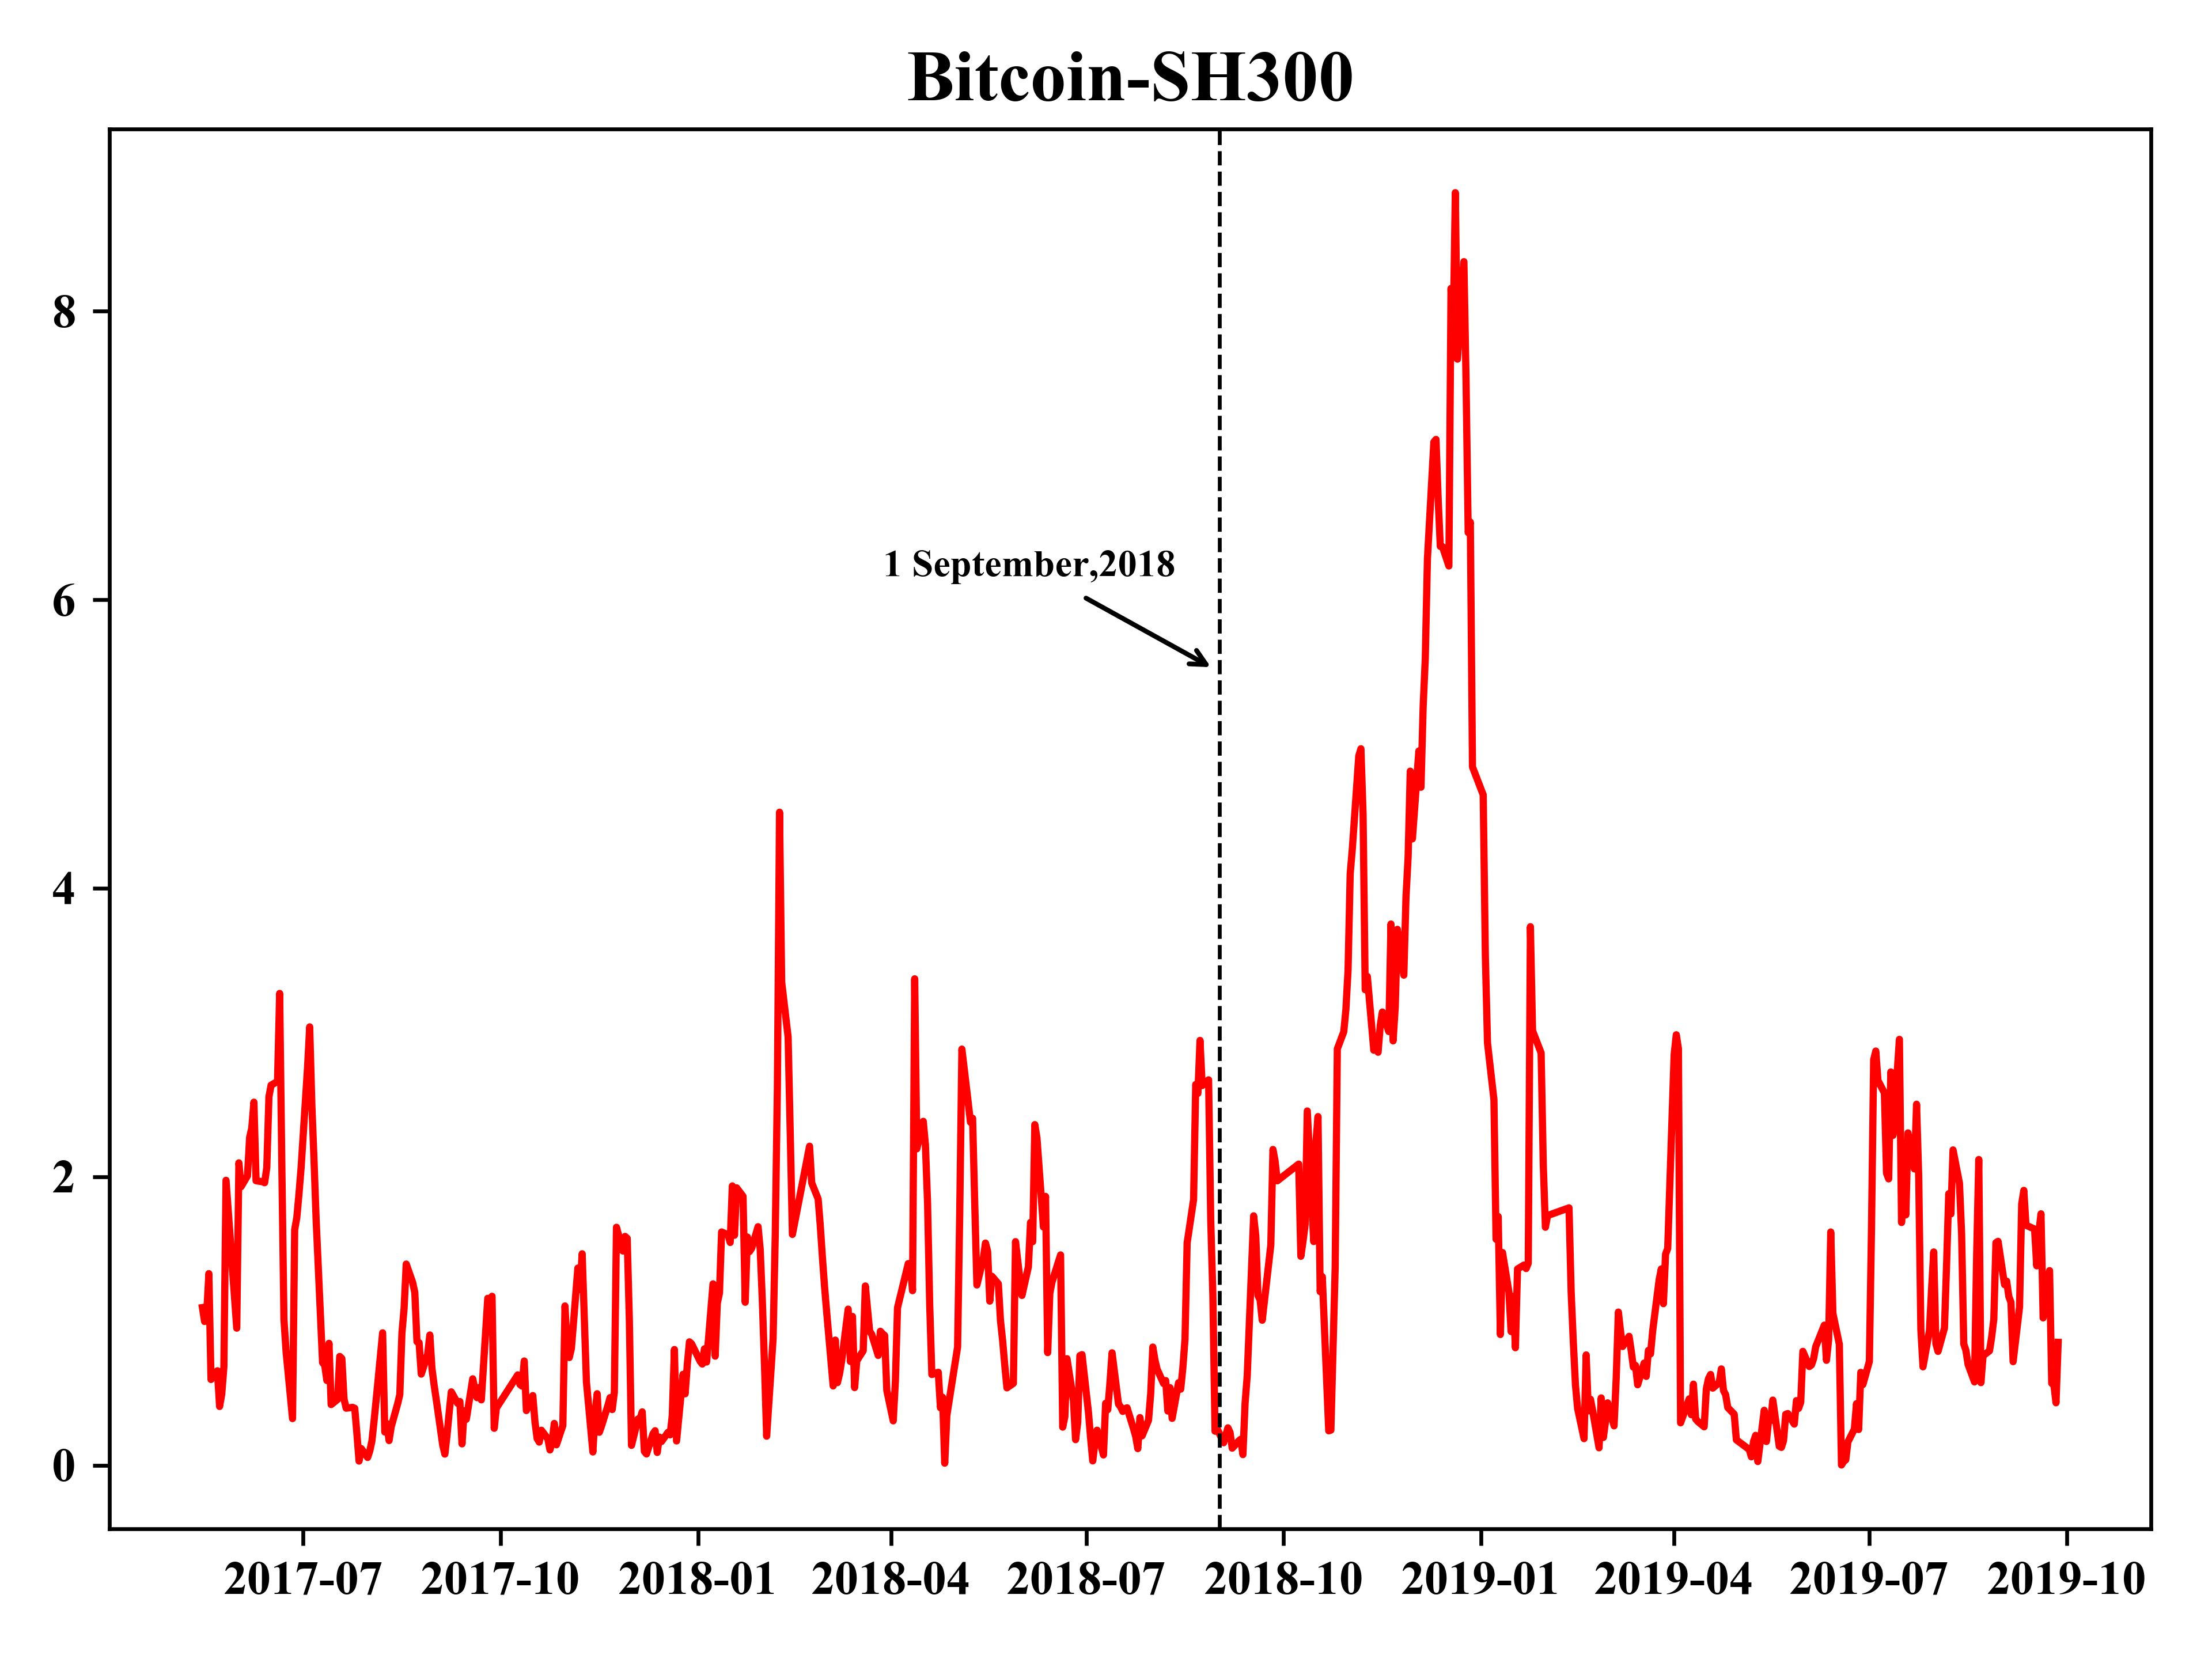
\includegraphics[width=0.45\textwidth]{SH300.png}}
	\subfigure[NPVS of SH300]{
		\label{SH300.sub.2}
		\includegraphics[width=0.45\textwidth]{SH300-Net.png}}
	
	\caption{The correlation and net pairwise volatility spillover of SH300}
	\label{SH300.main}
\end{figure}

Following Figure \ref{SH300.sub.1}, the correlation sharply increases in the early second stage. At the same time, the net pairwise volatility spillover of Bitcoin and SH300 has a obviously directional fluctuation. Furthermore, the direction of shocks is changes, while the volatility spillover increases. (see Figure \ref{SH300.sub.1}) This may reveal that domestic investors may use Bitcoin for hedging risks of Sino-US trade dispute. From a portfolio perspective, Bitcoin will accelerate the opening up of China's financial markets. However, noting that the other stock indexes barely change from Table \ref{tab4}. This shows that the other capital markets are opened enough. Hence the investors present little interest in Bitcoin. In addition, it also explains that Bitcoin is not a investable assets but a currency for payment attribute. As Figure \ref{SH300.sub.1} presents, the driving factors of the relationship may be different on account of the disparate performance between two stages



\subsubsection{Bitcoin Dollarization?}
For Forex markets, focusing on the United States' currency, the volatility between Bitcoin and USDX has no significant differences in two stages (see 17th row in \ref{tab4}), which is further strengthened that Bitcoin do not be dollarized. As plotted in Figure \ref{USDX.sub.2}, the relative strength of volatility spillover is always changes during while period. In addition, the correlation mostly fluctuates, which may show the connection is not stable. 

\begin{figure}[H]
	\centering  %图片全局居中
	
	\subfigure[Correlation of USDX]{
		\label{USDX.sub.1}
		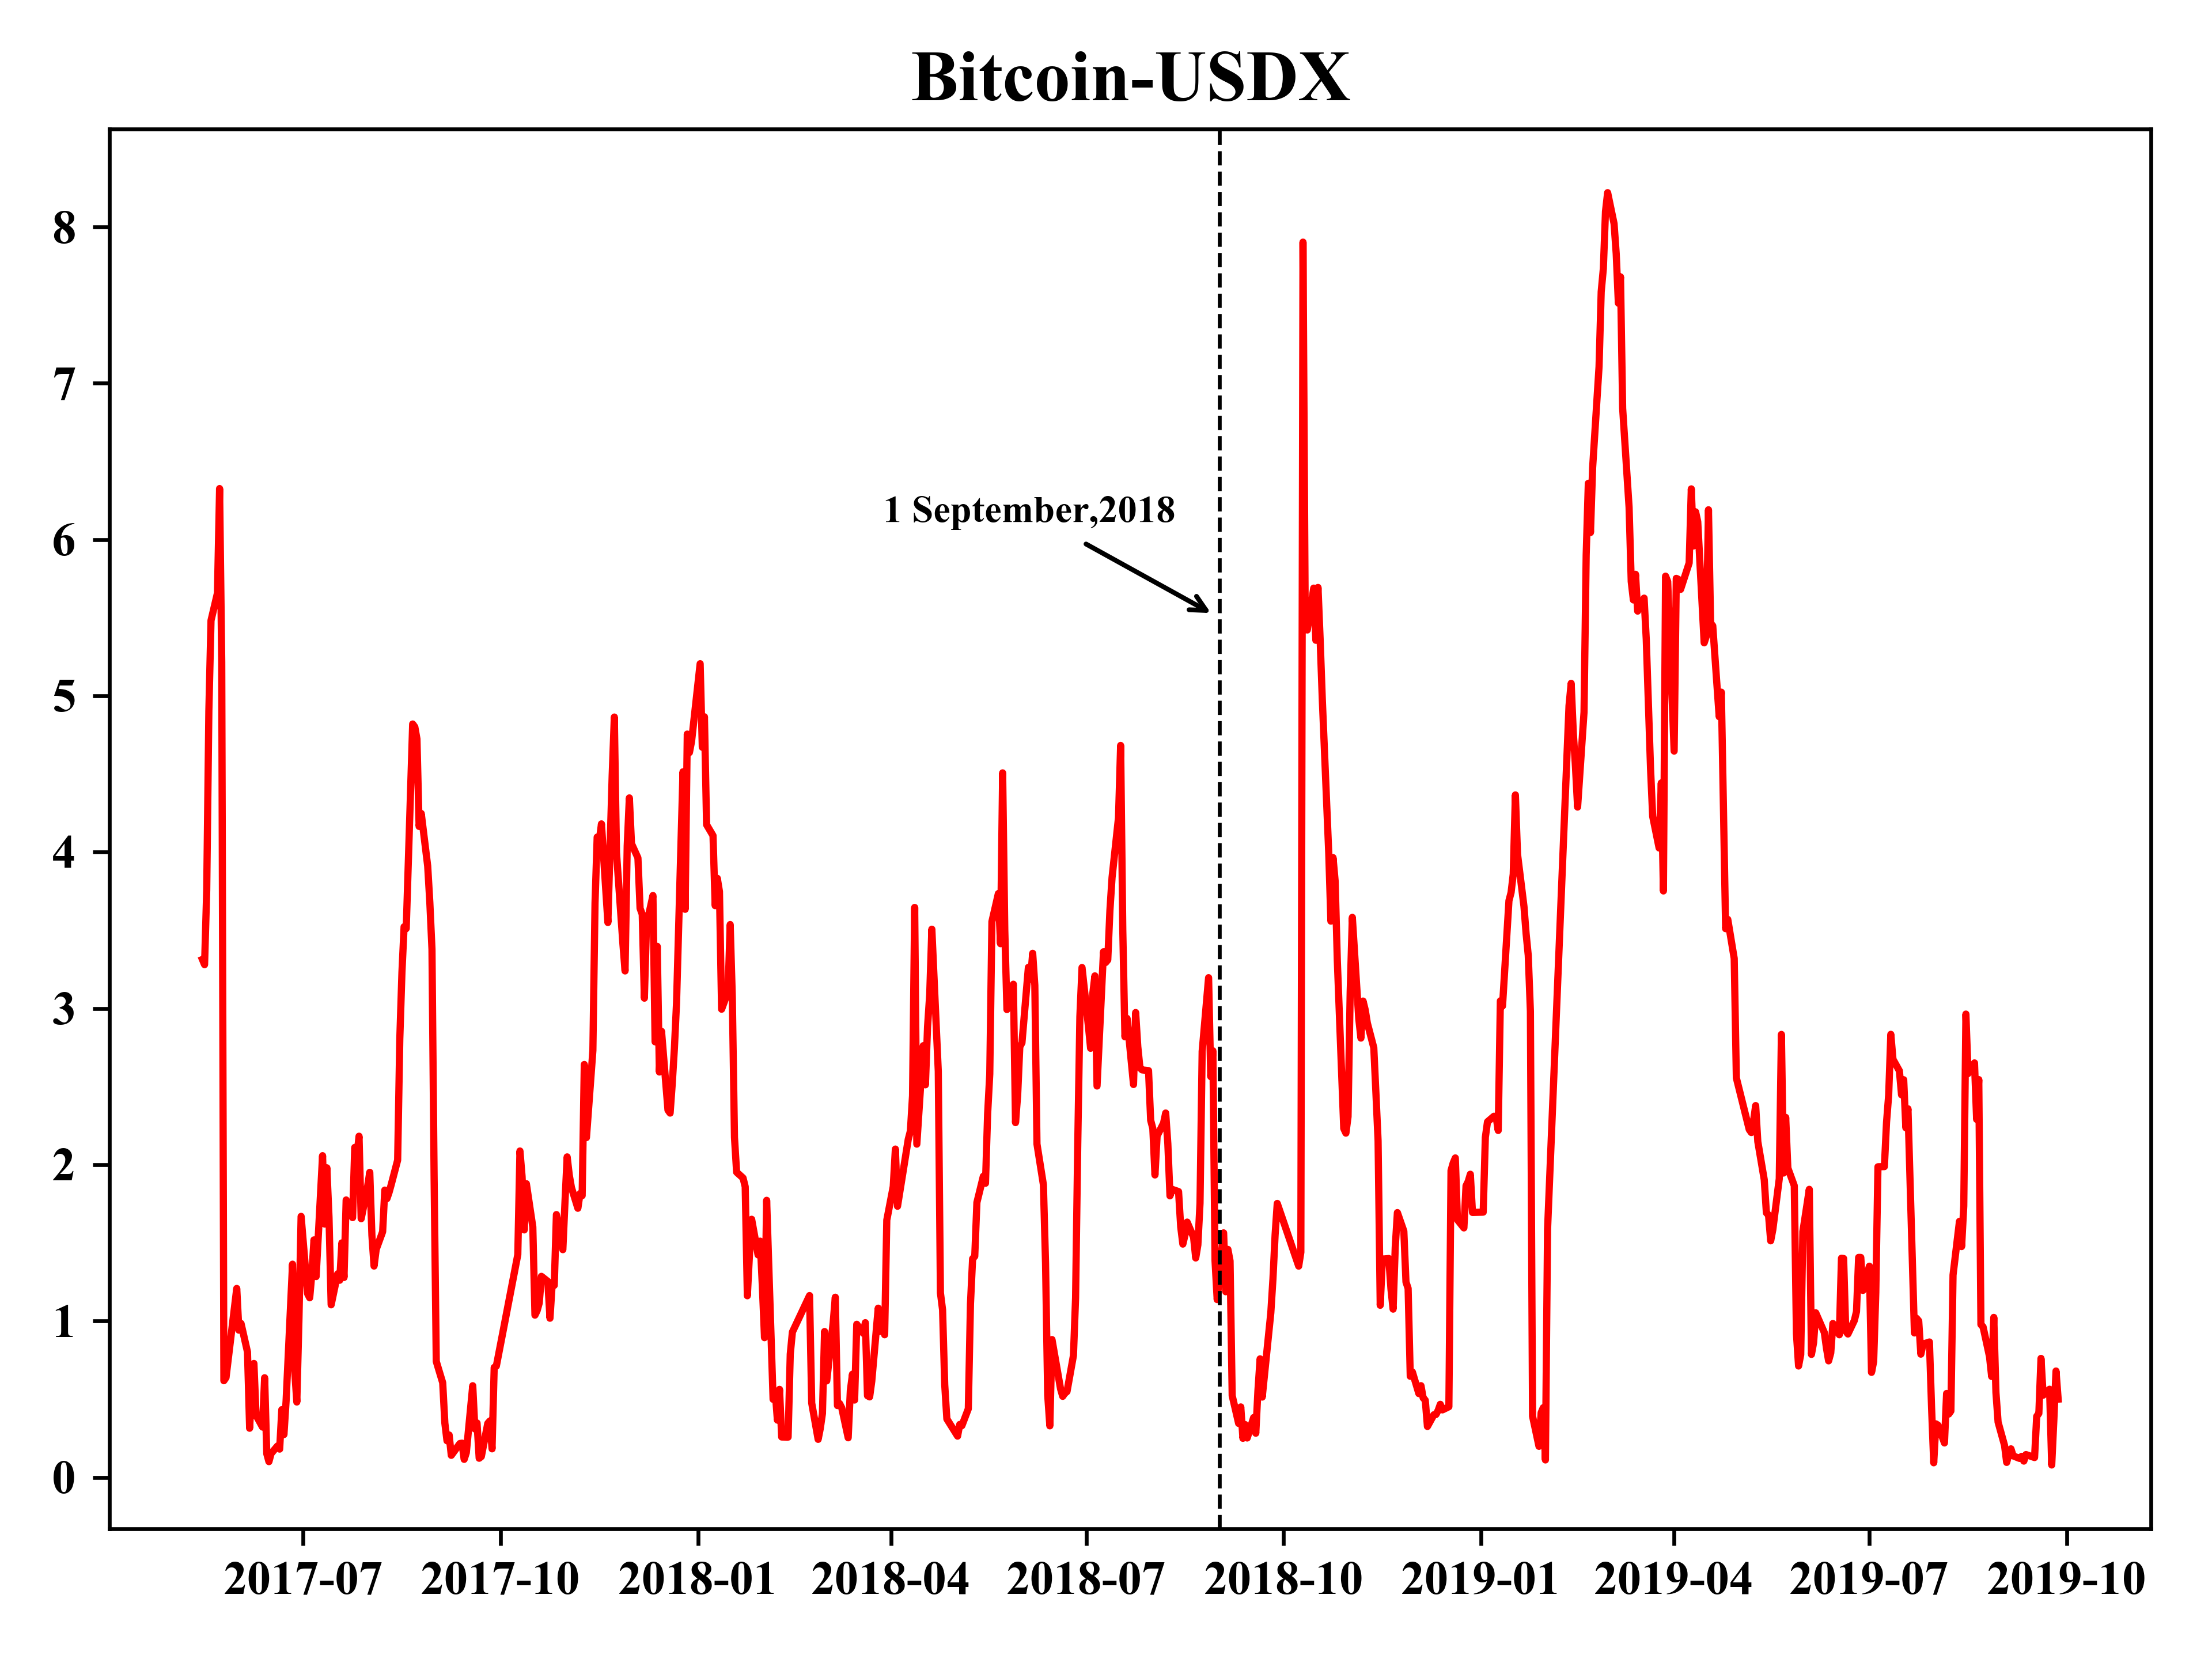
\includegraphics[width=0.45\textwidth]{USDX.png}}
	\subfigure[NPVS of USDX]{
		\label{USDX.sub.2}
		\includegraphics[width=0.45\textwidth]{USDX-Net.png}}

	\caption{The correlation and net pairwise volatility spillover of USDX}
	\label{USDX.main}
\end{figure}




\subsection{Robustness Analysis}
\subsubsection{DCC-GARCH Model}
As \ref{tab2} indicates, the ARCH effect of UFE and GUE is significant. Therefore, applying DCC-GARCH Model, these two variables, which is worth studying, are revealed the robust. \footnote{GUE is always a primary volatility contributor in two stages. For instance, 21.14\% (2.74 / 12.96) in the first stage, and 12.58\% (3.14 / 24.96) in another stage. In addition, the correlatedness of UFE is the biggest in Forex markets. See 13th row of Table \ref{tab4}}

\begin{figure}[H]
	\centering  %图片全局居中
	
	\subfigure[Dynamic Correlation of UFE]{
		\label{DCC.sub.1}
		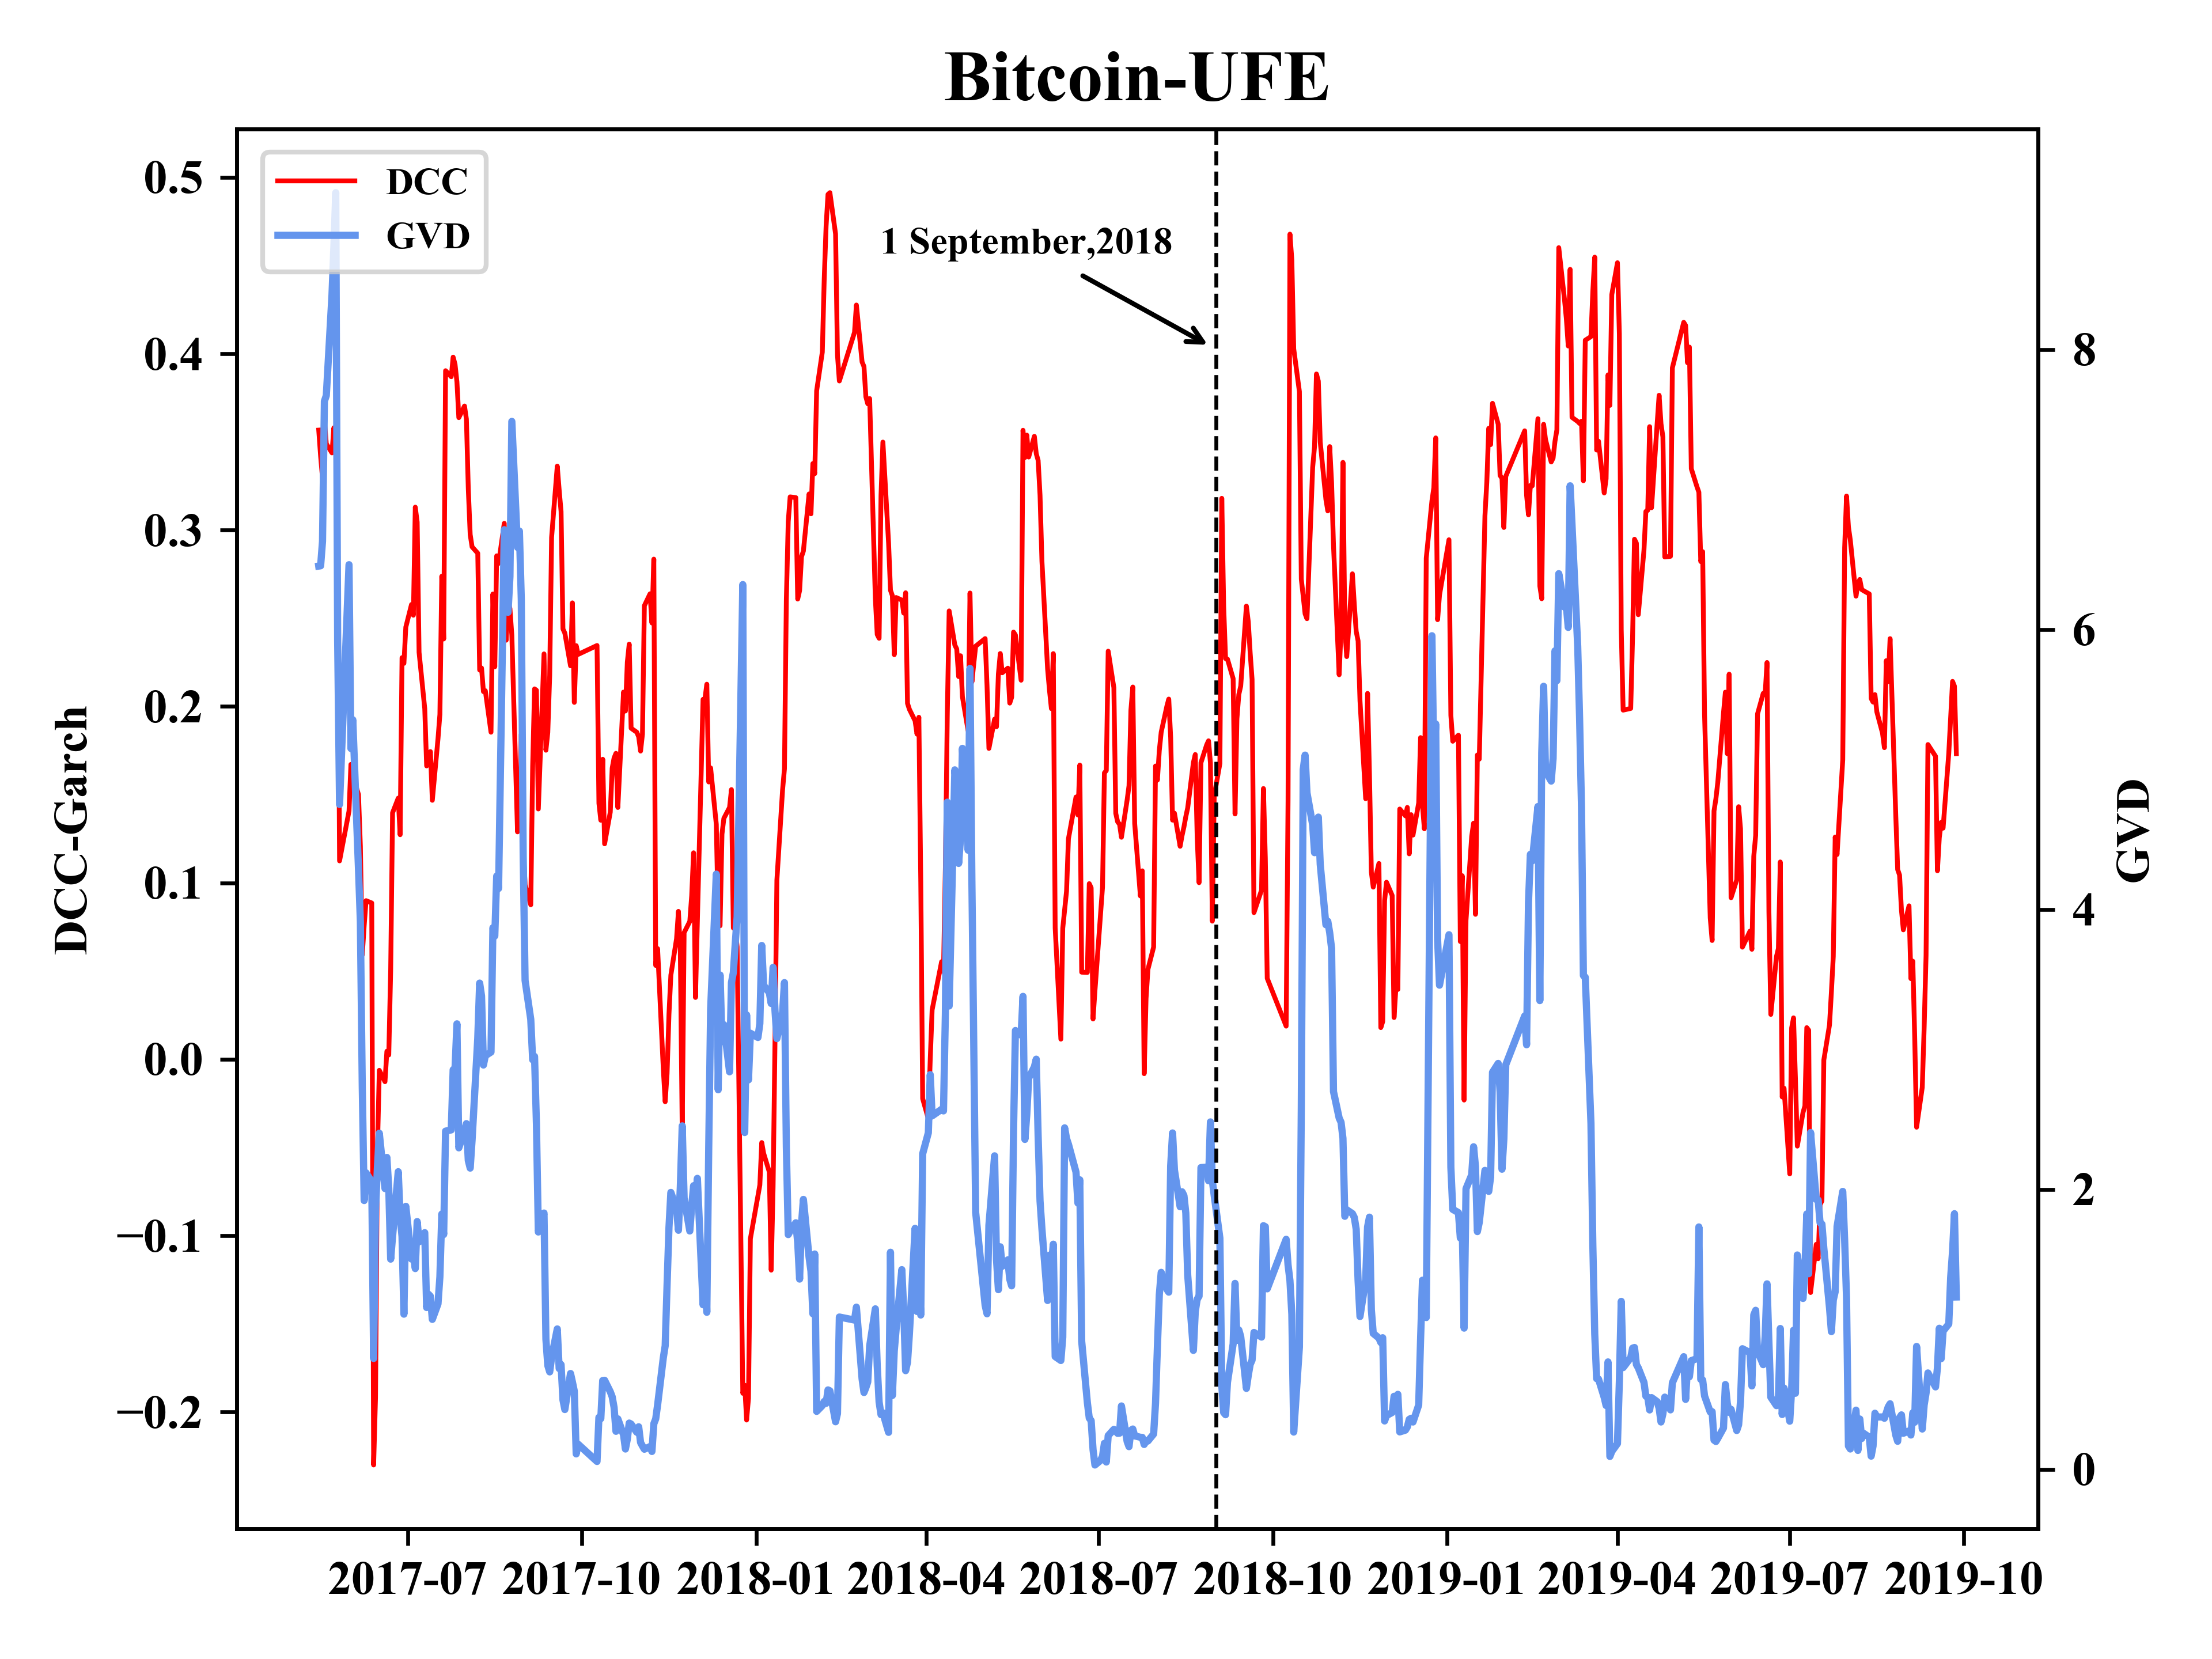
\includegraphics[width=0.45\textwidth]{UFE-DCC-GVD.png}}
	\subfigure[Dynamic Correlation of GUE]{
		\label{DCC.sub.2}
		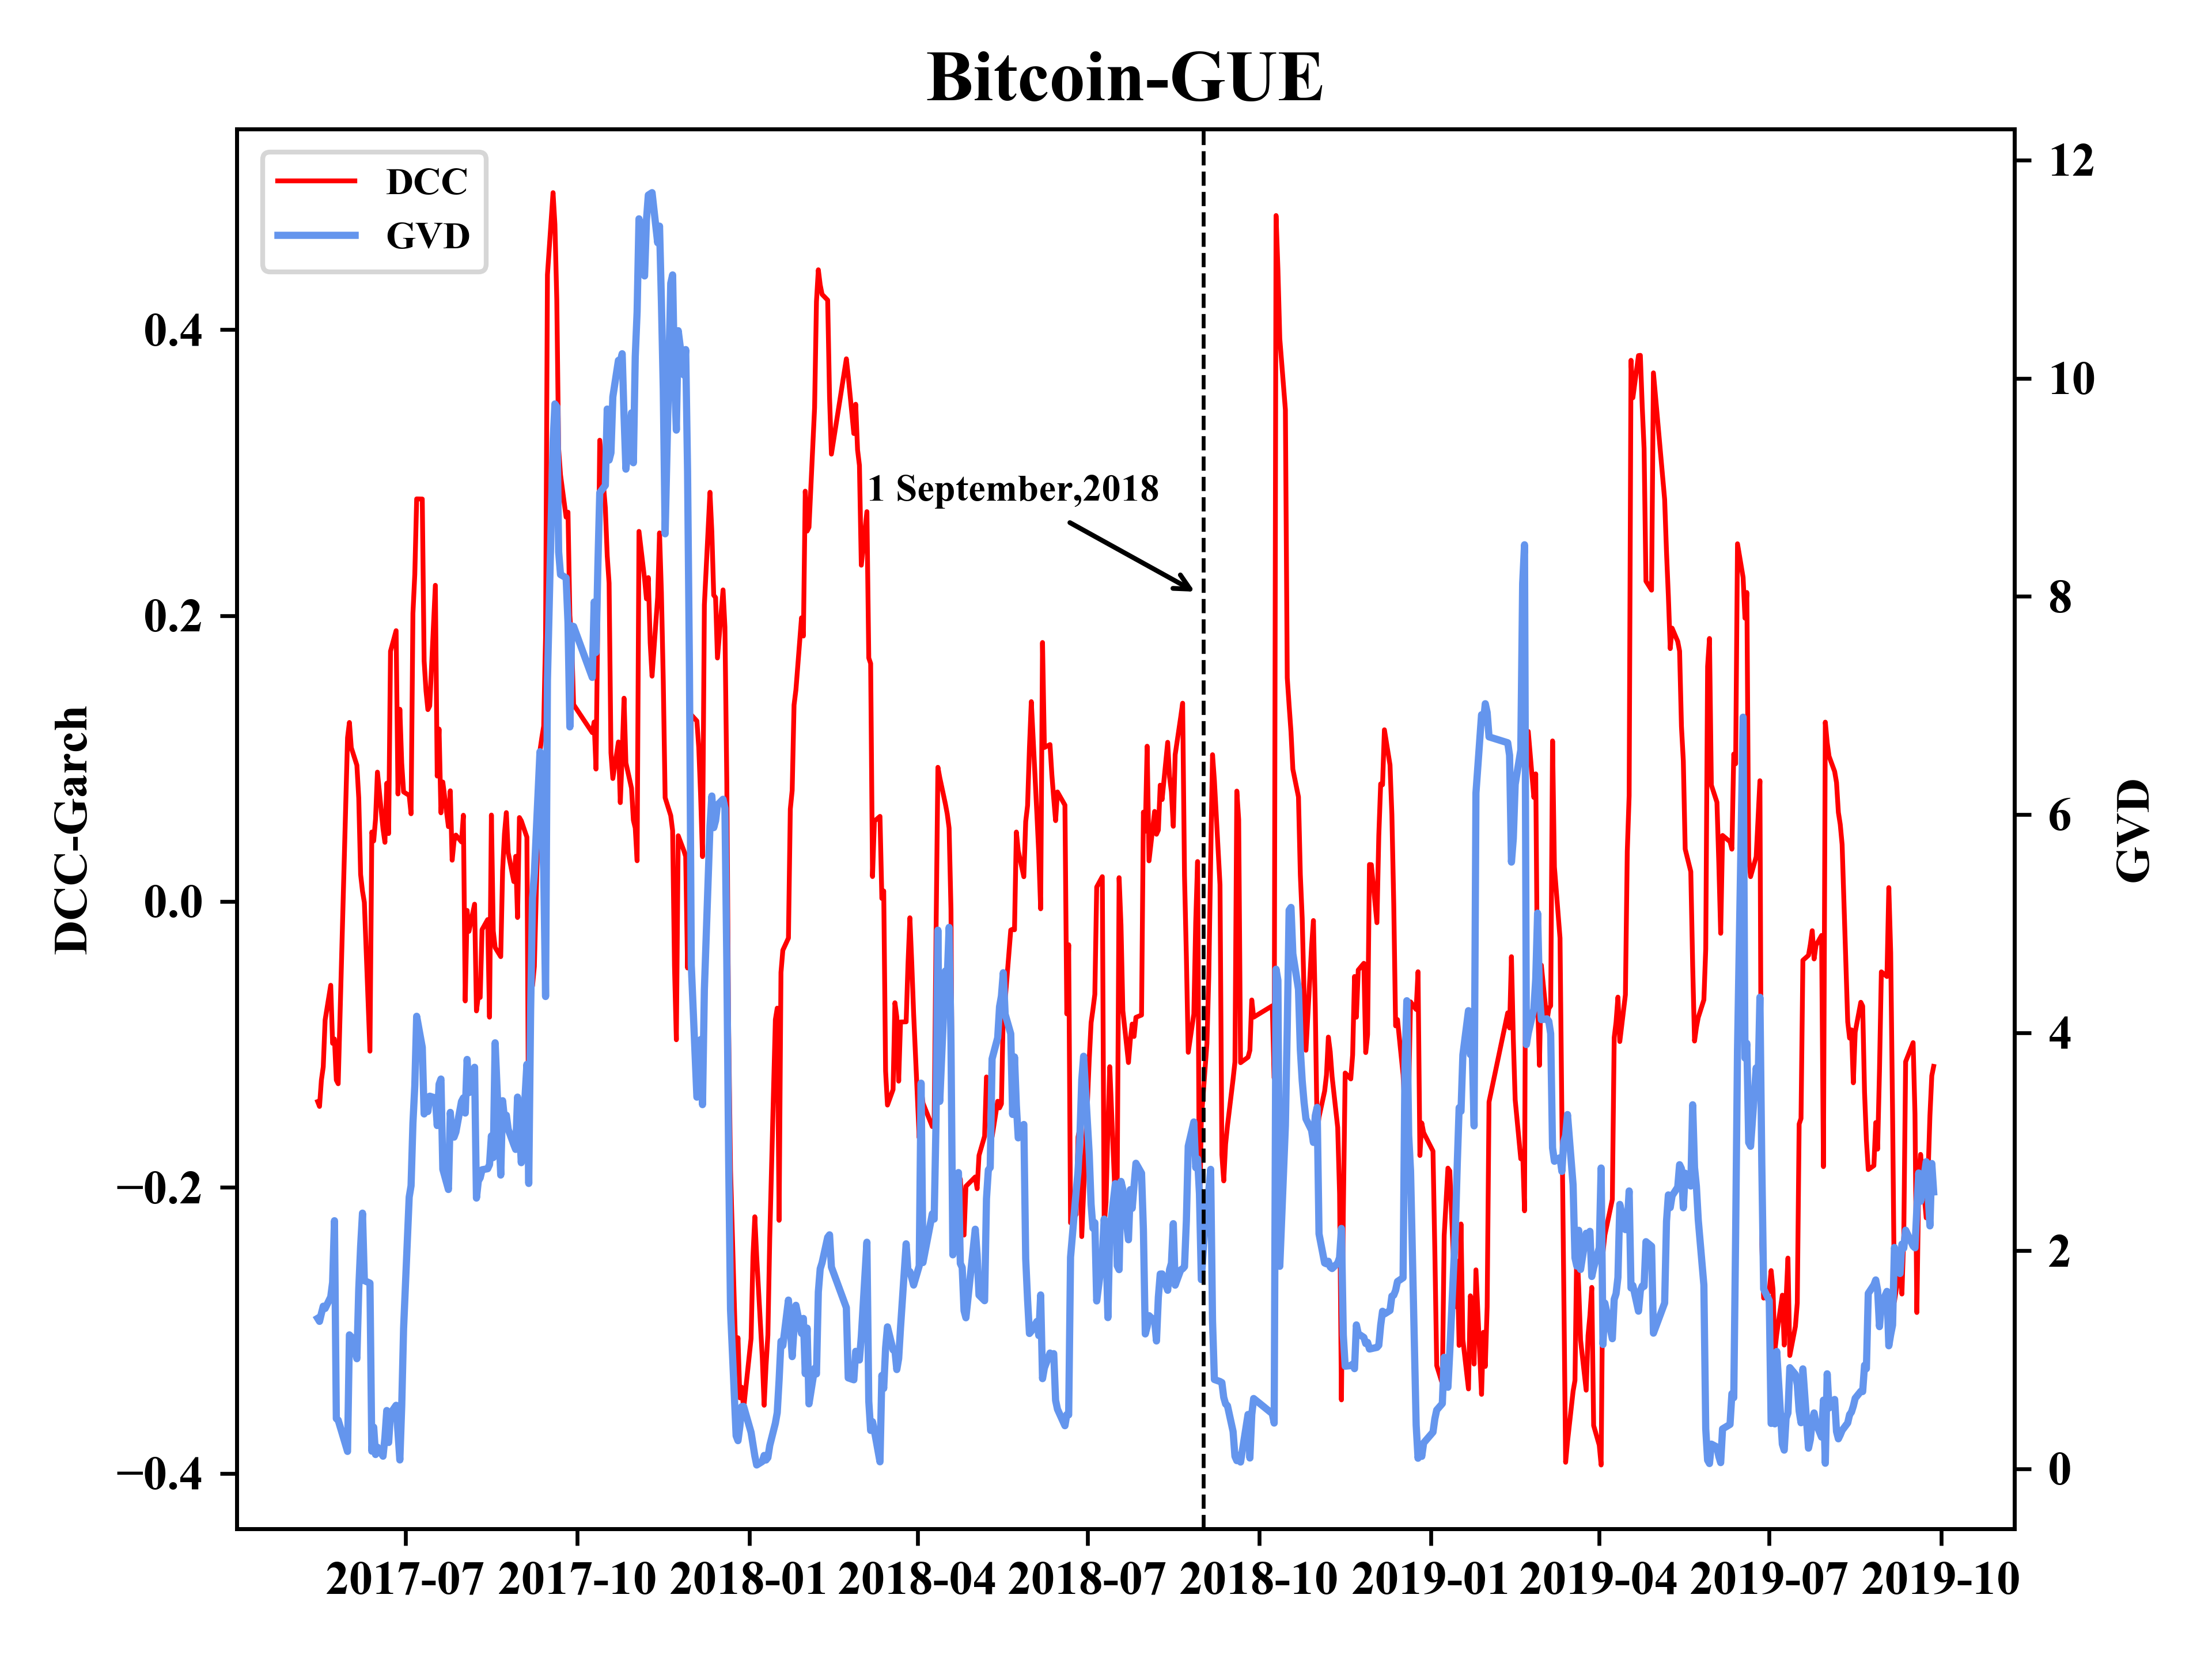
\includegraphics[width=0.45\textwidth]{GUE-DCC-GVD.png}}
	
	\caption{The dynamic correlation of GUE and UFE in two methods}
	\label{DCC.main}
\end{figure}


Following Figure \ref{DCC.main}, first look at the overall similarity before we dive into details of. It is obvious that two quite different methods obtain nearly similar trend. In addition, the data of DCC-GARCH Model is more smooth. (see red curve in Figure \ref{DCC.sub.1} and \ref{DCC.sub.2}) Now, we turn to carefully compare these two methods. First of all, the trend of UFE is more similar in the second phase, and the similarity of two curves in Figure \ref{DCC.sub.2} is bigger in the early stage, respectively. Additionally, the significant difference appears during the period from January 2018 to April 2018. Finally, the UFE' average correlation is higher than that of GUE, which corresponds with conclusions from Table \ref{tab4}. Furthermore, we quantitatively study these conclusions in Table \ref{tab5}. For daily frequency data, the full-sample correlations reveal that the estimated correlations in our paper are reliable.

\begin{table}[]
	\centering
	\setlength{\abovecaptionskip}{0pt}%    
	\setlength{\belowcaptionskip}{10pt}%
	\caption{Correlation of Dynamic correlation produced by two methods}
	\renewcommand\tabcolsep{30 pt}
	\label{tab5}
	\scalebox{0.65}{
		\begin{tabular}{ccc}
			\hline
			& UFE & GUE \\
			\hline
			UFE\_DCC & 0.1696*** & 0.0866** \\
			GUE\_DCC & -0.1639*** & 0.2821*** \\
			\hline
		\end{tabular}
	}
\end{table}

\subsubsection{Granger Test}
As Table \ref{tab6} shows, Bitcoin is significant negative correlated with SH300. This corresponds to the fact that the volatility spillover of SH300 to Bitcoin is bigger than the opposite direction. (see 6th row Table \ref{tab4}). In addition, these safe-haven assets, such as UFE, UJE and UFG, are significant related to Bitcoin, which has been demonstrated for several methods in our paper.

\begin{table}[]
	\centering
	\setlength{\abovecaptionskip}{0pt}%    
	\setlength{\belowcaptionskip}{10pt}%
	\caption{Correlation of Daily Volatility}
	\renewcommand\tabcolsep{5 pt}
	\label{tab6}
	\scalebox{0.65}{
		\begin{tabular}{cccccccccc}
			\hline
			& SH300 & SP500 & USDX & ISG & IFG & DFG & UFE & UJE & GUE \\
			\hline
			First Stage & 0.0011 & 0.0021 & 0.0004 & 0.004 & 0.0155 & 0.0227 & 0.1793*** & 0.0671 & 0.1209** \\
			Second Stage & -0.2025*** & 0.0614 & -0.0896 & 0.1525** & 0.2015*** & 0.2410*** & 1.007 & 0.108 & -0.1418* \\
			All Sample & -0.1716*** & 0.0909** & 0.0384 & 0.0571 & 0.0760* & 0.0351 & 0.1983*** & 0.1289*** & -0.0139 \\
			\hline
		\end{tabular}
	}
\end{table}


Hence, we turn to study the Granger-Cause test reported in Table \ref{tab7}. Firstly, Bitcoin is the Granger cause of SH300, which means that Bitcoin is the net volatility contributor to SH300. Subsequently, UFE and UJE has a bidirectional Granger cause with Bitcoin. This emerges that the volatilities of the two safe-haven currencies are bidirectional lead relations. Finally, there are not Granger cause between gold assets and Bitcoin. This phenomenon reveals that Bitcoin becomes a safe-haven asset like gold assets, but its volatility do not attribute to gold assets. Therefore, Bitcoin's safe-haven attribute is because of its scarcity, like gold assets.


\begin{table}[]
	\centering
	\setlength{\abovecaptionskip}{0pt}%    
	\setlength{\belowcaptionskip}{10pt}%
	\caption{Correlation of Daily Volatility}
	\renewcommand\tabcolsep{10 pt}
	\label{tab7}
	\scalebox{0.65}{
		\begin{tabular}{cccccccc}
			\hline
			& \multicolumn{3}{c}{H$_0$:Other assets do not Granger-cause Bitcoin} &  & \multicolumn{3}{c}{H$_0$:Bitcoin do not Granger-cause other assets} \\
			\cline{2-4}
			\cline{6-8}
			& All Sample & First Stage & Second Stage &  & All Sample & First Stage & Second Stage \\
			\hline
			SH300 & 1.13 & 0.61 & 0.41 &  & 6.57** & 0.14 & 7.46*** \\
			SP500 & 0.48 & 0.62 & 0.15 &  & 0.59 & 1.55 & 0.17 \\
			USDX & 5.50** & 2.49 & 0.25 &  & 4.53** & 0.24 & 0.02 \\
			ISG & 0.24 & 0.03 & 1.22 &  & 0.01 & 0.24 & 0.66 \\
			IFG & 0.40 & 0.45 & 0.52 &  & 0.77 & 0.98 & 0.41 \\
			DFG & 0.01 & 0.00 & 1.8 &  & 0.01 & 0.21 & 0.76 \\
			UFE & 8.41*** & 3.39* & 1.87 &  & 10.59*** & 3.45* & 1.35 \\
			UJE & 4.66** & 0.12 & 2.03 &  & 414.70*** & 0.38 & 3.95** \\
			GUE & 1.37 & 3.46* & 0.03 &  & 0.57 & 0.83 & 0.00 \\
			\hline
		\end{tabular}
	}
	
\end{table}

Table \ref{tab7} indicates that in the first phase, UFE is nearly the only cause of Bitcoin, and Bitcoin has little influence to other assets. In addition, the volatility spillovers, presented in Table \ref{tab4}, also confirms that Bitcoin is little correlated with other assets. Furthermore, the figures of correlations, such as Figure \ref{Gold.main}, Figure \ref{Currency.main} and Figure \ref{SH300.main}, strengthen this conclusion. Therefore, Bitcoin do bot become an investible asset until 1 September, 2018. And before then, Bitcoin is more like a speculative asset.


\section{Conclusions and Implications}
This paper sheds further light on investigating the connectedness within cryptocurrency market and conventional financial markets, including gold, stocks and currencies. With applying the generalized spectral representation variance decomposition approach as proposed by \cite{Diebold2012} and \cite{Bariviera2017}, we believe that Bitcoin is becoming a safe-haven asset on account of the economic uncertainty caused by Sino-US trade dispute. In addition, several interesting conclusions are proposed. Firstly, this nascent markets of cryptocurrencies did not become investible, such as hedging risks, until the beyond expectation tariff was imposed. And after then, the connectedness between safe-haven assets, such as golds, CHF and JPY, sharply increased. Secondly, SH300 is further related with Bitcoin, and Bitcoin significantly brings about some of the volatility. This wound drive China's financial markets opening up whether this connectedness obtains continued progress. Finally, we argue that cryptocurrencies were dollarized. While the relatedness increases, the direction of influence is unstable. Furthermore, the bidirectional Granger-Cause reveals that driving orientation is uncertain. Therefore, cryptocurrencies have not been nationalized.


Based on the previous findings and conclusions, we propose some recommendations for investors,  regulators and policymakers as follows. For investors, digital currency assets allocations should be more careful due to the absence of nationalization. Hence, this asset is more likely to be speculative. For regulators, regarding huge market cap and trade volume of Bictoin, incorporating digital currency into the regulatory scope as soon as possible is conducive to the healthy development of cryptocurrencies. For policymakers, especially for the Chinese government, cryptocurrencies have become a volatility contributor of stock markets, and this will disguisedly drive financial markets opening up without strategic planing. Hence, strengthening the supervisionin of cryptocurrencies is of great significance in the process of financial openness.


Our research also has some limitations for further studies. Firstly, the economic mechanism that Bitcoin influences SH300 should be elaborated, which will reveal the crucial driving factors during the development of cryptocurrencies. Subsequently, there is no solid theoretical basis for the determination of some parameters, such as the lag intervals for endogenous. Finally, we should study different sampling periods, including weekly frequency data. As fluctuation reduces, more interesting conclusions will be reported.


\bibliography{MyCollection.bib}
\end{document}
 






